%------ENTREGABLES------
%codigo pipeline funcionando
%archivos .mem para:
%test de pruebas para las instrucciones del cuadro 1
% - programa ISA sin dependencias

%-------INFORME-------
%1. breve resumen del pipeline: datapath, control
%2. implementacion de instrucciones(cuadro 1)
% - descripcion de cambios en el codigo
% - diagrama de datapath final
%3. Programa isa sin dependencias
%4. waveform
%5. mostrar con resultados intermedios que el programa funciona correctamente

\documentclass[11pt,a4paper]{article}

\usepackage[utf8]{inputenc}
\usepackage[T1]{fontenc}
\usepackage[margin=2.5cm]{geometry}
\usepackage{graphicx}
\usepackage{booktabs}
\usepackage{xcolor}
\usepackage{float}
\usepackage{listings}
\usepackage{enumitem}
\usepackage[plainpages=false,pdfpagelabels]{hyperref}

\hypersetup{colorlinks=true, linkcolor=blue, urlcolor=blue}

\renewcommand{\tablename}{Cuadro}
\renewcommand{\figurename}{Figura}
\renewcommand{\partname}{Parte}
\renewcommand{\thepart}{\arabic{part}}

\definecolor{codegray}{gray}{0.5}
\definecolor{codeblue}{rgb}{0.0,0.0,0.6}
\lstdefinestyle{verilog}{
  language=Verilog,
  basicstyle=\ttfamily\scriptsize,
  keywordstyle=\color{codeblue}\bfseries,
  commentstyle=\color{codegray}\itshape,
  numbers=none,
  frame=single,
  breaklines=true,
  showstringspaces=false,
  tabsize=2,
  aboveskip=4pt,
  belowskip=4pt
}
\lstset{style=verilog}

\title{Procesador RISC-V Segmentado (Pipeline)\\\large Arquitectura de Computadoras --- Semana 13}
\author{Steve Andy Ildefonso Santos}
\date{\today}

\begin{document}

% ============================================================
% PORTADA: pagina en blanco reservada para completar a mano
% (nombres, titulo, curso, docente, logo, etc.)
% ============================================================
{\thispagestyle{empty}
\centering
\vspace*{2cm}

\includegraphics[width=0.45\textwidth]{utec_logo.jpg}

\vfill
{\Huge\bfseries Implementación de procesador RISC-V\par}
\vfill

\begin{tabular}{|l|c|}
	\hline
	\textbf{Nombre y apellidos}     & \textbf{Código de estudiante} \\
	\hline
	Steve Andy Ildefonso Santos     & 202410402                     \\
	\hline
	Miguel Luis Paucar Barrios      & 202410276                     \\
	\hline
	Marcelo Mateo Rosillo Rodríguez & 202410597                     \\
	\hline
\end{tabular}

\vfill
{\large Perú - 2026\par}
\vspace{1cm}
\clearpage}

\part{Procesador segmentado y unidad de riesgos}

\section{Resumen teórico del pipeline: datapath y control}

La \textbf{segmentación} (\textit{pipelining}) es una técnica que aumenta el
rendimiento de un procesador dividiendo la ejecución de una instrucción en varias
\textbf{etapas} secuenciales, cada una a cargo de un segmento de hardware dedicado y
separada de la siguiente por un \textbf{registro de pipeline}. Al igual que en una
línea de ensamblaje, varias instrucciones se ejecutan a la vez, cada una en una etapa
distinta.

La segmentación \textbf{no reduce la latencia} de una instrucción individual (de
hecho puede aumentarla ligeramente por el retardo de los registros), pero sí
incrementa el \textbf{throughput}: en el caso ideal se completa una instrucción por
ciclo. Además, el periodo de reloj queda determinado por la etapa más lenta y no por
el datapath completo, por lo que puede ser mucho menor que en una organización
\textit{single-cycle}.

En el RISC-V clásico se emplean \textbf{cinco etapas}:

\begin{table}[ht]
	\centering
	\begin{tabular}{@{}llll@{}}
		\toprule
		\textbf{Etapa} & \textbf{Sigla} & \textbf{Función}                                     & \textbf{Registro de salida} \\
		\midrule
		Fetch          & F              & Lee la instrucción de memoria; incrementa el PC      & IF/ID                       \\
		Decode         & D              & Decodifica; lee el banco de registros; extiende imm. & ID/EX                       \\
		Execute        & E              & Realiza la operación de la ALU; calcula saltos       & EX/MEM                      \\
		Memory         & M              & Lee o escribe en la memoria de datos                 & MEM/WB                      \\
		Writeback      & W              & Escribe el resultado en el banco de registros        & ---                         \\
		\bottomrule
	\end{tabular}
	\caption{Las cinco etapas del pipeline RISC-V y su registro de frontera.}
\end{table}

\subsection{Datapath}

La ruta de datos segmentada se obtiene \textbf{cortando} el datapath
\textit{single-cycle} en las cinco etapas anteriores e insertando registros de
pipeline entre ellas. Estos registros tienen una doble función: por un lado dividen
el camino crítico (acortando el periodo de reloj) y por otro \textbf{mantienen cada
	valor asociado a su instrucción} mientras esta avanza una etapa por ciclo.

Así, en cada registro de frontera se guarda todo lo que las etapas posteriores
necesitarán de esa instrucción: la propia instrucción, el contador de programa
(\texttt{PC} y \texttt{PC+4}), los operandos leídos del banco de registros, el
inmediato extendido, el número de registro destino y los resultados de la ALU o de la
memoria. Una idea central es que \textbf{todas las señales de una misma instrucción
	deben avanzar en conjunto}; por ejemplo, el número de registro destino debe
propagarse por todas las etapas hasta llegar al Writeback sincronizado con su dato.

\subsection{Control}

La \textbf{unidad de control} decodifica la instrucción en la etapa Decode y genera
las señales que gobiernan el datapath (selección de operandos, operación de la ALU,
escritura en memoria, escritura en el banco de registros, control del salto, etc.).

El punto clave de la teoría es que muchas de esas señales \textbf{se generan en
	Decode pero se utilizan en etapas posteriores}: por ejemplo, la señal de escritura en
memoria se usa en Memory, y la de escritura en registros, en Writeback. Por lo tanto,
las señales de control deben \textbf{segmentarse igual que los datos}, viajando a
través de los registros de pipeline hasta la etapa exacta en la que actúan. De este
modo el camino de control replica la estructura por etapas del datapath y cada señal
llega junto con el dato al que corresponde.

\subsection{Riesgos (\textit{hazards})}

El precio de la segmentación son los \textbf{riesgos}: situaciones en las que una
instrucción no puede ejecutarse en el ciclo siguiente porque depende de información
que aún no está disponible. Al haber varias instrucciones simultáneamente en el
pipeline, los resultados y las decisiones de salto no siempre están listos a tiempo.
Se clasifican en tres tipos:

\begin{itemize}
	\item \textbf{De datos:} una instrucción necesita el resultado de otra anterior que
	      todavía no ha terminado de escribirse en el banco de registros. Es el caso
	      \textit{lectura-tras-escritura} (RAW): mientras la instrucción productora
	      sigue avanzando por el pipeline, la consumidora ya leyó un valor antiguo. Un
	      caso particularmente crítico es el \textit{load-use}, cuando una instrucción
	      usa de inmediato el dato que una carga (\texttt{lw}) todavía no ha traído de
	      memoria.
	\item \textbf{De control:} los saltos (\texttt{beq}, \texttt{jal}, \texttt{jalr},
	      etc.) se resuelven en una etapa tardía (Execute). Para entonces ya se han
	      captado (\textit{fetch}) las instrucciones que seguían secuencialmente, que
	      podrían no ser las correctas si el salto se toma. Cada salto tomado introduce
	      así una penalización de ciclos.
	\item \textbf{Estructurales:} dos etapas requieren el mismo recurso de hardware en
	      el mismo ciclo. En este diseño se evitan separando la memoria de instrucciones
	      de la de datos (Fetch y Memory no compiten) y permitiendo que el banco de
	      registros se escriba y se lea en el mismo ciclo.
\end{itemize}

Estos riesgos se resuelven con una \textbf{unidad de riesgos} que combina tres
mecanismos: \textit{forwarding} (adelantar un resultado desde una etapa posterior a la
que lo necesita, sin esperar al Writeback), \textit{stalls} (detener el pipeline unos
ciclos cuando el adelanto no basta, como en el \textit{load-use}) y \textit{flush}
(anular las instrucciones mal captadas tras un salto tomado). De forma provisional
---mientras no exista dicha unidad--- los riesgos se evitan insertando instrucciones
\texttt{NOP} entre las instrucciones dependientes, que es el enfoque usado en esta
fase del proyecto.

\begin{figure}[ht]
	\centering
	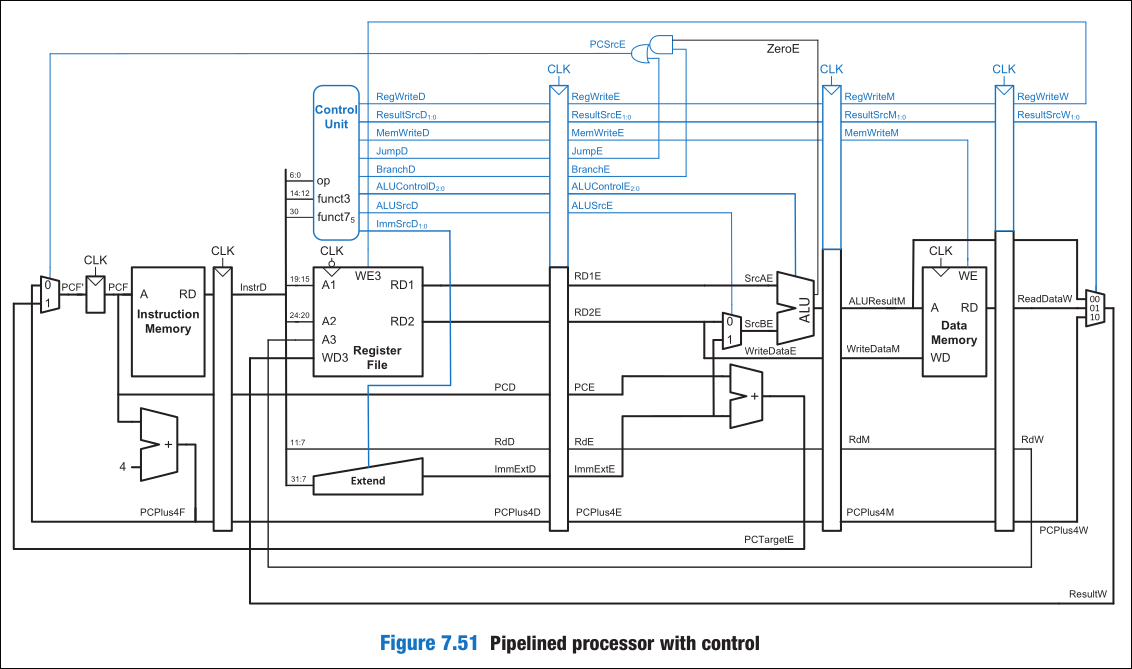
\includegraphics[width=\textwidth]{pipeline_diagram.png}
	\caption{Procesador RISC-V segmentado con control: las cinco etapas
		(Fetch, Decode, Execute, Memory y Writeback) separadas por registros de pipeline,
		y la unidad de control cuyas señales se segmentan hasta la etapa en que se usan.
		Fuente: Harris \& Harris, \textit{Digital Design and Computer Architecture,
			RISC-V Edition}, Figura~7.51.}
	\label{fig:pipeline}
\end{figure}

\section{Implementación de las instrucciones}

A partir del pipeline base (Figura~\ref{fig:pipeline}) se implementó el conjunto de
instrucciones del Cuadro~\ref{cuadro:isa}. La mayor parte de los cambios se concentró
en la \textbf{decodificación y el control}; la ruta de datos se reutilizó casi
íntegra, añadiendo únicamente las señales necesarias para los saltos condicionales y
\texttt{jalr}.

\subsection{Conjunto de instrucciones objetivo}

\begin{table}[ht]
	\centering
	\begin{tabular}{|l|l|}
		\hline
		\textbf{Instrucción}          & \textbf{Descripción}             \\
		\hline
		\texttt{lw rd, imm(rs1)}      & Load word                        \\ \hline
		\texttt{addi rd, rs1, imm}    & Add immediate                    \\ \hline
		\texttt{slli rd, rs1, shamt}  & Shift left logical immediate     \\ \hline
		\texttt{xori rd, rs1, imm}    & XOR immediate                    \\ \hline
		\texttt{srli rd, rs1, shamt}  & Shift right logical immediate    \\ \hline
		\texttt{srai rd, rs1, shamt}  & Shift right arithmetic immediate \\ \hline
		\texttt{ori rd, rs1, imm}     & OR immediate                     \\ \hline
		\texttt{andi rd, rs1, imm}    & AND immediate                    \\ \hline
		\texttt{sw rs2, imm(rs1)}     & Store word                       \\ \hline
		\texttt{add rd, rs1, rs2}     & Add                              \\ \hline
		\texttt{sub rd, rs1, rs2}     & Subtract                         \\ \hline
		\texttt{sll rd, rs1, rs2}     & Shift left logical               \\ \hline
		\texttt{xor rd, rs1, rs2}     & XOR                              \\ \hline
		\texttt{srl rd, rs1, rs2}     & Shift right logical              \\ \hline
		\texttt{sra rd, rs1, rs2}     & Shift right arithmetic           \\ \hline
		\texttt{or rd, rs1, rs2}      & OR                               \\ \hline
		\texttt{and rd, rs1, rs2}     & AND                              \\ \hline
		\texttt{lui rd, imm}          & Load upper immediate             \\ \hline
		\texttt{beq rs1, rs2, offset} & Branch if equal                  \\ \hline
		\texttt{bne rs1, rs2, offset} & Branch if not equal              \\ \hline
		\texttt{blt rs1, rs2, offset} & Branch if less than              \\ \hline
		\texttt{bge rs1, rs2, offset} & Branch if greater than or equal  \\ \hline
		\texttt{jalr rd, rs1, imm}    & Jump and link register           \\ \hline
		\texttt{jal rd, offset}       & Jump and link                    \\ \hline
	\end{tabular}
	\caption{Conjunto de instrucciones implementado (Cuadro 1).}
	\label{cuadro:isa}
\end{table}

\subsection{Fases de implementación}

El conjunto no se implementó de golpe, sino de forma \textbf{incremental y por
	familias funcionales}, partiendo de una base \textit{single-cycle} y convirtiéndola
primero a pipeline. Tras cada fase se validó con un \textit{testbench} independiente, y
después de los cambios grandes se reejecutó toda la batería de pruebas
(\textit{regresión}) para detectar regresiones. El Cuadro~\ref{cuadro:fases} resume el
proceso.

\begin{table}[ht]
	\centering
	\begin{tabular}{@{}cll@{}}
		\toprule
		\textbf{Fase} & \textbf{Objetivo}                           & \textbf{Instrucciones / cambio}                                                     \\
		\midrule
		1             & Arquitectura pipeline base                  & 5 etapas, registros, control segmentado, burbuja                                    \\
		2             & Subset mínimo (validar estructura)          & \texttt{add}, \texttt{addi}, \texttt{lw}, \texttt{sw}                               \\
		3             & Extender la ALU básica                      & \texttt{and}, \texttt{or}, \texttt{andi}, \texttt{ori}, \texttt{slt}, \texttt{slti} \\
		4             & Lógica XOR                                  & \texttt{xor}, \texttt{xori}                                                         \\
		5             & Control de flujo básico                     & \texttt{beq}, \texttt{jal}                                                          \\
		6             & Inmediato superior                          & \texttt{lui}                                                                        \\
		7             & \texttt{ALUControl} a 4 bits + shifts       & \texttt{sll}, \texttt{srl}, \texttt{sra} (y sus \textit{imm})                       \\
		8             & Familia de branches                         & \texttt{bne}, \texttt{blt}, \texttt{bge}                                            \\
		9             & Salto a registro                            & \texttt{jalr}                                                                       \\
		10            & \textit{Register file} \textit{write-first} & puente hacia la fase de \textit{hazards}                                            \\
		\bottomrule
	\end{tabular}
	\caption{Fases de implementación del conjunto de instrucciones.}
	\label{cuadro:fases}
\end{table}

Tres decisiones guiaron el proceso: (i)~construir \textbf{primero el pipeline base},
luego el ISA y al final los \textit{hazards}, para aislar el origen de cualquier fallo;
(ii)~\textbf{reutilizar el datapath} siempre que fuera posible, concentrando los cambios
en el control; y (iii)~validar con \textbf{pruebas separadas por familia} más una
regresión completa tras cada cambio estructural (por ejemplo, al ampliar
\texttt{ALUControl} a 4 bits).

\subsection{Resumen de los cambios por módulo}

\begin{table}[ht]
	\centering
	\begin{tabular}{@{}ll@{}}
		\toprule
		\textbf{Módulo}       & \textbf{Qué se modificó}                                                       \\
		\midrule
		\texttt{maindec.v}    & Nuevos \textit{opcodes} (lui, jalr, jal); \texttt{default} como burbuja        \\
		\texttt{aludec.v}     & \texttt{ALUControl} ampliado a 4 bits; decode de shifts, branches y lui        \\
		\texttt{alu.v}        & Nuevas operaciones: xor, slt, lui (pasa B), sll, srl, sra                      \\
		\texttt{extend.v}     & Inmediato tipo U/J compartiendo \texttt{ImmSrc=11}                             \\
		\texttt{controller.v} & \texttt{funct3} segmentado; \texttt{PCSrcE} para la familia de branches y jalr \\
		\texttt{datapath.v}   & \texttt{CondBitE}, destino de \texttt{jalr} y mux de \texttt{PCTarget}         \\
		\texttt{regfile.v}    & Escritura \textit{write-first} (flanco de bajada)                              \\
		\bottomrule
	\end{tabular}
	\caption{Módulos modificados respecto al pipeline base.}
\end{table}

\subsection{Decodificador principal (\texttt{maindec.v})}

Se agregaron los \textit{opcodes} de \texttt{lui}, \texttt{jalr} y \texttt{jal}, junto
con un nuevo bit de control \texttt{Jalr}. El caso \texttt{default} genera una burbuja
segura (todas las señales en cero), evitando valores \texttt{x} durante el llenado del
pipeline.

\begin{lstlisting}
// RegWrite_ImmSrc_ALUSrc_MemWrite_ResultSrc_Branch_ALUOp_Jump_Jalr
7'b0110111: controls = 12'b1_11_1_0_00_0_11_0_0; // lui
7'b1100111: controls = 12'b1_00_1_0_10_0_00_0_1; // jalr
7'b1101111: controls = 12'b1_11_0_0_10_0_00_1_0; // jal
default:    controls = 12'b0_00_0_0_00_0_00_0_0; // burbuja / nop
\end{lstlisting}

\subsection{Decodificador de la ALU (\texttt{aludec.v}) y \texttt{ALUControl}}

La señal \texttt{ALUControl} se amplió de 3 a 4 bits para dar cabida a las nuevas
operaciones (shifts y \texttt{lui}) sin reciclar códigos. La nueva codificación es:

\begin{table}[ht]
	\centering
	\begin{tabular}{@{}cl@{}}
		\toprule
		\textbf{ALUControl} & \textbf{Operación} \\
		\midrule
		\texttt{0000}       & add                \\
		\texttt{0001}       & sub                \\
		\texttt{0010}       & and                \\
		\texttt{0011}       & or                 \\
		\texttt{0100}       & xor                \\
		\texttt{0101}       & slt                \\
		\texttt{0110}       & lui (pasa B)       \\
		\texttt{0111}       & sll                \\
		\texttt{1000}       & srl                \\
		\texttt{1001}       & sra                \\
		\bottomrule
	\end{tabular}
	\caption{Codificación de \texttt{ALUControl} (4 bits).}
\end{table}

El decode distingue los shifts por \texttt{funct3} y \texttt{funct7b5}, y los branches
\texttt{blt}/\texttt{bge} usan \texttt{slt}:

\begin{lstlisting}
2'b01: if (funct3 == 3'b100 || funct3 == 3'b101)
         ALUControl = 4'b0101;   // blt, bge -> slt
       else
         ALUControl = 4'b0001;   // beq, bne -> sub
2'b11:   ALUControl = 4'b0110;   // lui (pasa B)
default: case(funct3)            // R-type / I-type
  3'b001: ALUControl = 4'b0111;  // sll, slli
  3'b101: ALUControl = funct7b5 ? 4'b1001 : 4'b1000; // sra/srai : srl/srli
  3'b100: ALUControl = 4'b0100;  // xor, xori
  // ...
endcase
\end{lstlisting}

\subsection{ALU (\texttt{alu.v})}

Se añadieron los casos correspondientes a las nuevas operaciones; los desplazamientos
toman la cuenta de los 5 bits menos significativos del operando B, y \texttt{sra} usa
desplazamiento aritmético con extensión de signo.

\begin{lstlisting}
4'b0100: result = a ^ b;                  // xor
4'b0110: result = b;                      // lui (pasa el inmediato)
4'b0111: result = a << b[4:0];            // sll
4'b1000: result = a >> b[4:0];            // srl
4'b1001: result = $signed(a) >>> b[4:0];  // sra
\end{lstlisting}

\subsection{ALU modificada: vista interna}

La Figura~\ref{fig:alu-modificada} muestra el interior de la ALU (basada en la
Figura~5.18(b) de Harris \& Harris, que ya soporta \texttt{slt} con corrección de
\textit{overflow}) con las operaciones añadidas resaltadas en \textbf{rojo}: la
compuerta \texttt{xor} (código \texttt{0100}), el paso directo de \texttt{lui}
(código \texttt{0110}, el inmediato \texttt{B} sin modificar) y el bloque
\texttt{Shifter} con sus tres salidas \texttt{sll}/\texttt{srl}/\texttt{sra}
(códigos \texttt{0111}/\texttt{1000}/\texttt{1001}). El multiplexor de salida
creció de 5 a 10 entradas y \texttt{ALUControl} pasó de 3 a 4 bits para poder
direccionarlas.

\begin{figure}[H]
	\centering
	\includegraphics[width=\textwidth]{alu_modificada.pdf}
	\caption{ALU interna con las operaciones añadidas resaltadas en rojo: \texttt{xor},
		\texttt{lui} y el \textit{shifter} (\texttt{sll}/\texttt{srl}/\texttt{sra}). Las
		operaciones base (\texttt{add}, \texttt{sub}, \texttt{and}, \texttt{or}, \texttt{slt})
		se conservan sin cambios.}
	\label{fig:alu-modificada}
\end{figure}

\subsection{Extensor de inmediato (\texttt{extend.v})}

Se añadió \texttt{op} como entrada para compartir \texttt{ImmSrc=11} entre \texttt{lui}
(inmediato tipo U) y \texttt{jal} (tipo J), desambiguando por el \textit{opcode}:

\begin{lstlisting}
2'b11: if (op == 7'b0110111)
         immext = {instr[31:12], 12'b0};                 // lui (U)
       else
         immext = {{12{instr[31]}}, instr[19:12],
                   instr[20], instr[30:21], 1'b0};        // jal (J)
\end{lstlisting}

\subsection{Control de saltos (\texttt{controller.v})}

Para la familia de branches se segmentó \texttt{funct3} hasta la etapa Execute
(\texttt{funct3E}) y se redefinió \texttt{PCSrcE} para cubrir \texttt{beq}, \texttt{bne},
\texttt{blt}, \texttt{bge} y \texttt{jalr}:

\begin{lstlisting}
assign PCSrcE = JumpE | JalrE |
                (BranchE & (
                  (funct3E == 3'b000 &  ZeroE)    |  // beq
                  (funct3E == 3'b001 & ~ZeroE)    |  // bne
                  (funct3E == 3'b100 &  CondBitE) |  // blt
                  (funct3E == 3'b101 & ~CondBitE)    // bge
                ));
\end{lstlisting}

\subsection{Ruta de datos (\texttt{datapath.v})}

En Execute se expuso \texttt{CondBitE} (bit~0 del resultado de la ALU, usado por
\texttt{blt}/\texttt{bge}) y se calculó el destino de \texttt{jalr} con el bit~0 forzado
a cero; un mux selecciona entre el destino de salto relativo y el de \texttt{jalr}:

\begin{lstlisting}
assign CondBitE      = ALUResultE[0];
assign PCJalrTargetE = {ALUResultE[31:1], 1'b0};
assign PCTargetE     = JalrE ? PCJalrTargetE : PCBranchTargetE;
\end{lstlisting}

\subsection{Banco de registros (\texttt{regfile.v})}

El banco de registros es el punto de realimentación del pipeline: se \textbf{lee en
	Decode} pero se \textbf{escribe en Writeback}. Esto genera un riesgo de datos de
``distancia~3'': cuando una instrucción que está en Writeback escribe un registro que
otra instrucción, situada en Decode, lee en el \textbf{mismo ciclo}.

Si la escritura se hace en el \textbf{flanco de subida} (\textit{posedge}), la
escritura y la lectura ocurren en el mismo flanco; con la semántica de asignación no
bloqueante, la lectura captura el valor \textbf{antiguo} y la instrucción dependiente
recibe un dato obsoleto. Por eso se eligió la escritura \textbf{write-first} en el
\textbf{flanco de bajada} (\textit{negedge}): el resultado se escribe en la primera
mitad del ciclo y queda disponible para leerse en la segunda mitad del \textbf{mismo}
ciclo.

\begin{lstlisting}
always @(negedge clk)
  if (we3) rf[a3] <= wd3;
\end{lstlisting}

Se eligió este cambio por tres razones teóricas: (i)~es la organización que el libro
especifica para el banco de registros del procesador segmentado (Sección~7.5.1);
(ii)~\textbf{resuelve el riesgo de distancia~3 en el propio banco de registros}, de
modo que la futura unidad de riesgos solo deberá cubrir las distancias~1 y~2 (cuando el
resultado aún está en las etapas Execute o Memory), simplificando la lógica de
\textit{forwarding}; y (iii)~es un cambio mínimo y no destructivo, que no altera el
resto del datapath.

\subsection{Diagrama de datapath final}

La Figura~\ref{fig:datapath-final} muestra el \textit{datapath} completo del
pipeline con la implementación de instrucciones, incluyendo la Unidad de Control y
las señales que se propagan por los registros de pipeline (en azul). Las
adiciones específicas de este proyecto respecto al pipeline base de Harris \&
Harris se marcan en \textbf{rojo}: la señal \texttt{Jalr} (que viaja como
\texttt{JalrD}$\to$\texttt{JalrE}), la señal \texttt{funct3} propagada por
separado hasta Execute (\texttt{funct3E}, necesaria para distinguir
\texttt{beq}/\texttt{bne}/\texttt{blt}/\texttt{bge}), \texttt{ALUControl}
ampliado a 4 bits, y el multiplexor que selecciona entre
\texttt{PCBranchTargetE} y \texttt{PCJalrTargetE} según \texttt{JalrE} para
calcular \texttt{PCTargetE}.

\begin{figure}[H]
	\centering
	\includegraphics[width=\textwidth]{datapath_final.pdf}
	\caption{Datapath final del pipeline con la Unidad de Control (señales en azul) y
		las adiciones específicas del proyecto en rojo: \texttt{Jalr}, \texttt{funct3E},
		\texttt{ALUControl} de 4 bits y el multiplexor de destino de \texttt{jalr}.}
	\label{fig:datapath-final}
\end{figure}

\subsection{Validación: testbenches por familia}
\label{sec:tests}

En vez de un único test gigante, cada familia funcional se validó con un
\textit{testbench} y un programa de prueba independientes. Esto \textbf{aísla los
	errores}: si un cambio rompía algo, se detectaba de inmediato y con contexto. Cada
programa usa \texttt{NOP} entre las instrucciones dependientes (todavía no hay unidad de
riesgos) y escribe resultados a memoria, que el \textit{testbench} compara con los
valores esperados. El Cuadro~\ref{cuadro:tests} resume la cobertura.

\begin{table}[ht]
	\centering
	\begin{tabular}{@{}ll@{}}
		\toprule
		\textbf{Testbench}          & \textbf{Instrucciones cubiertas}                                                                                                           \\
		\midrule
		\texttt{testbench\_base}    & \texttt{add}, \texttt{addi}, \texttt{lw}, \texttt{sw}, \texttt{and}, \texttt{or}, \texttt{andi}, \texttt{ori}, \texttt{slt}, \texttt{slti} \\
		\texttt{testbench\_ctrl}    & \texttt{beq}, \texttt{jal}                                                                                                                 \\
		\texttt{testbench\_xor}     & \texttt{xor}, \texttt{xori}                                                                                                                \\
		\texttt{testbench\_lui}     & \texttt{lui}                                                                                                                               \\
		\texttt{testbench\_shift}   & \texttt{sll}, \texttt{slli}, \texttt{srl}, \texttt{srli}, \texttt{sra}, \texttt{srai}                                                      \\
		\texttt{testbench\_branch3} & \texttt{bne}, \texttt{blt}, \texttt{bge}                                                                                                   \\
		\texttt{testbench\_jalr}    & \texttt{jalr}                                                                                                                              \\
		\bottomrule
	\end{tabular}
	\caption{Testbenches por familia funcional y las instrucciones que validan.}
	\label{cuadro:tests}
\end{table}

Todos los testbenches se ejecutan con un único comando de regresión
(\texttt{make test}), que compila y corre cada uno reportando \texttt{PASS}/\texttt{FAIL}.
Tras cada cambio estructural (por ejemplo, ampliar \texttt{ALUControl} a 4~bits) se
reejecutó toda la batería para descartar regresiones; el conjunto completo pasa
correctamente.

\section{Programa ISA sin dependencias}

Para comprobar que el procesador \textbf{ejecuta correctamente un programa real}, se
escribió un programa breve y \textbf{sin dependencias de datos cercanas}, de modo que
corre sobre el pipeline base \textbf{sin necesidad de insertar \texttt{NOP}}. El objetivo
no es ejercitar todas las instrucciones (eso lo cubren los \textit{testbenches} por
familia de la Sección~\ref{sec:tests}), sino mostrar el funcionamiento correcto de un
programa completo.

\subsection{Estrategia: ausencia de dependencias}

El programa primero carga \textbf{operandos independientes} en \texttt{x1}--\texttt{x4}
(cada uno a partir de \texttt{x0} y un inmediato, sin dependencia entre ellos). Luego
realiza tres operaciones que leen únicamente esos registros ---ya asentados--- y escriben
en registros nuevos, y finalmente guarda los resultados en memoria. Las operaciones se
ordenan de modo que ninguna lee un registro escrito menos de tres instrucciones antes,
por lo que \textbf{no se produce ningún riesgo de datos}.

\begin{lstlisting}[language={}]
addi x1, x0, 5     # x1 = 5
addi x2, x0, 7     # x2 = 7
addi x3, x0, 3     # x3 = 3
addi x4, x0, 10    # x4 = 10
add  x5, x1, x2    # x5 = 5 + 7  = 12
sub  x6, x2, x3    # x6 = 7 - 3  = 4
or   x7, x1, x4    # x7 = 5 | 10 = 15
sw   x5, 0(x0)     # Mem[0] = 12
sw   x6, 4(x0)     # Mem[4] = 4
sw   x7, 8(x0)     # Mem[8] = 15
\end{lstlisting}

\subsection{Resultados esperados}

El Cuadro~\ref{cuadro:resultados} lista los valores que el programa escribe en memoria.
Como no hay riesgos, los resultados son los aritméticamente correctos y el
\textit{testbench} los verifica uno a uno.

\begin{table}[ht]
	\centering
	\begin{tabular}{@{}clr@{}}
		\toprule
		\textbf{Dir.} & \textbf{Operación}      & \textbf{Valor} \\
		\midrule
		0             & \texttt{add x5, x1, x2} & 12             \\
		4             & \texttt{sub x6, x2, x3} & 4              \\
		8             & \texttt{or  x7, x1, x4} & 15             \\
		\bottomrule
	\end{tabular}
	\caption{Resultados del programa ISA sin dependencias
		(\texttt{x1}$=$5, \texttt{x2}$=$7, \texttt{x3}$=$3, \texttt{x4}$=$10).}
	\label{cuadro:resultados}
\end{table}

\subsection{Waveform}

La Figura~\ref{fig:waveform-isa} muestra la simulación del programa ISA sin
dependencias, capturada en GTKWave. En ella se aprecia el comportamiento esperado del
pipeline:

\begin{itemize}
	\item \textbf{Avance por etapas:} el número de registro destino aparece primero en
	      \texttt{RdD} y luego, un ciclo después, en \texttt{RdE}, \texttt{RdM} y
	      \texttt{RdW}. Se ve la secuencia \texttt{1,2,3,4,5,6,7} desplazándose
	      \textbf{en diagonal} (un escalón por ciclo): esa es la confirmación de que la
	      segmentación funciona y de que hay varias instrucciones en vuelo a la vez.
	\item \textbf{Flujo de instrucciones:} \texttt{InstrD} muestra una a una las diez
	      instrucciones del programa mientras \texttt{PCF} se incrementa de~4 en~4. Como
	      no hay \texttt{NOP}, las instrucciones se suceden \textbf{sin huecos} (pipeline
	      siempre llena).
	\item \textbf{Resultados:} \texttt{ALUResultE} muestra primero los operandos cargados
	      (\texttt{5, 7, 3, 10}) y luego los resultados de las operaciones
	      (\texttt{12}~$=$~\texttt{add}, \texttt{4}~$=$~\texttt{sub},
	      \texttt{15}~$=$~\texttt{or}).
	\item \textbf{Escrituras a memoria:} en los ciclos finales, cuando \texttt{MemWrite}
	      se activa, \texttt{WriteData} muestra los valores \texttt{12, 4, 15} que se
	      guardan en las direcciones \texttt{0, 4, 8}, coincidiendo con los resultados
	      esperados (Cuadro~\ref{cuadro:resultados}).
\end{itemize}

\begin{figure}[ht]
	\centering
	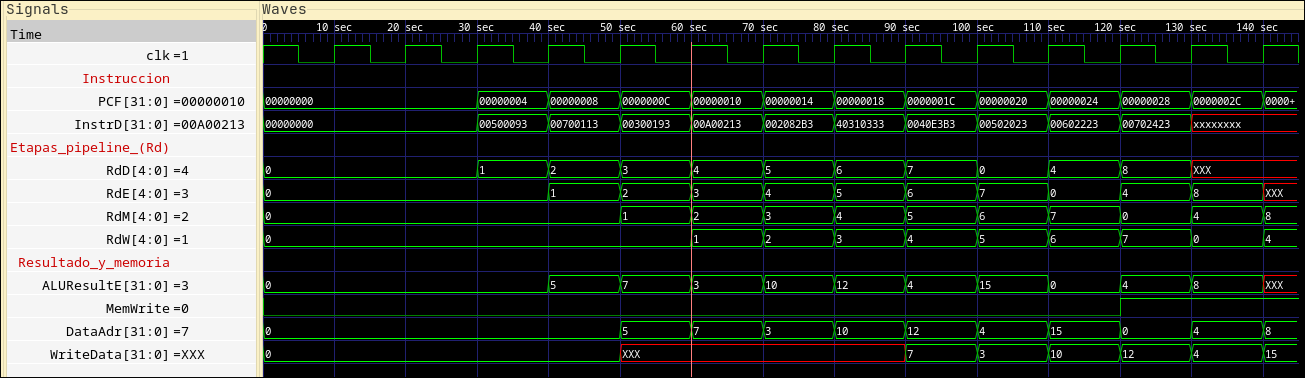
\includegraphics[width=\textwidth]{waveform_isa.png}
	\caption{Waveform del programa ISA sin dependencias. Se observa el avance en diagonal
		del registro destino (\texttt{RdD}$\to$\texttt{RdE}$\to$\texttt{RdM}$\to$\texttt{RdW}),
		el flujo de las instrucciones por el pipeline y la escritura de los resultados
		(\texttt{12, 4, 15}) en memoria.}
	\label{fig:waveform-isa}
\end{figure}

\subsection{Resultados intermedios y verificación}

\subsubsection{Los resultados intermedios coinciden con lo esperado}

La forma de onda de la Figura~\ref{fig:waveform-isa} permite seguir los resultados
\textbf{a medida que se calculan}, no solo al final. En la señal \texttt{ALUResultE}
aparecen, en orden, los valores producidos por la etapa Execute:

\begin{center}
	\texttt{5, 7, 3, 10} (carga de operandos) $\;\to\;$
	\texttt{12} (\texttt{add}), \texttt{4} (\texttt{sub}), \texttt{15} (\texttt{or}).
\end{center}

Un ciclo después, esos mismos valores viajan a la etapa Memory y, cuando
\texttt{MemWrite} se activa, se escriben en memoria: \texttt{WriteData} muestra
\texttt{12}, \texttt{4} y \texttt{15} en las direcciones \texttt{0}, \texttt{4}
y~\texttt{8}. Estos valores \textbf{coinciden exactamente} con los del
Cuadro~\ref{cuadro:resultados}.

El \textit{testbench} automatiza esta comprobación: en cada escritura a memoria compara
la dirección y el dato contra el valor esperado y, al coincidir los tres, imprime
\texttt{Simulation succeeded}. Que los resultados \textbf{intermedios} sean correctos
---y no solo el último--- demuestra que el procesador ejecuta el programa
correctamente en todas sus etapas.

\subsubsection{Cómo se ejecutan las pruebas}

La memoria de instrucciones (\texttt{imem}) carga su contenido desde el archivo
\texttt{riscvtest.mem} mediante \texttt{\$readmemh}. Por eso, cada prueba consiste en un
par \textbf{programa~(\texttt{.mem})~+~testbench~(\texttt{.v})}: se elige el programa de
la familia que se quiere validar, se copia como \texttt{riscvtest.mem} y se compila junto
con su \textit{testbench}. Por ejemplo, para validar los desplazamientos:

\begin{lstlisting}[language={}]
# 1. elegir el programa (lo carga imem via $readmemh)
cp tests/programs/riscvtest_shift.mem riscvtest.mem
# 2. compilar el diseno junto con el testbench de esa familia
iverilog -g2012 -o sim rtl/*.v tests/testbench_shift.v
# 3. ejecutar la simulacion
vvp sim
\end{lstlisting}

El \textit{script} de regresión (\texttt{make test}) automatiza este procedimiento para
\textbf{todas} las familias: por cada par copia el programa, compila con
\texttt{iverilog} y su \textit{testbench}, ejecuta con \texttt{vvp} y reporta
\texttt{PASS}/\texttt{FAIL}. La salida muestra que el conjunto completo pasa:

\noindent\begin{minipage}{\linewidth}
	\begin{lstlisting}[language={}]
--- Regresion pipeline RISC-V -------------------------
  base    PASS  Pipeline base subsets succeeded
  ctrl    PASS  Pipeline control subset succeeded
  xor     PASS  XOR subset ok: Mem[100] = 10
  lui     PASS  LUI subset ok: Mem[96] = 0x12345000
  shift   PASS  Shift subset succeeded
  branch  PASS  Branch family subset succeeded
  jalr    PASS  JALR subset succeeded
  deps    PASS  Simulation succeeded
  isa     PASS  Simulation succeeded
-------------------------------------------------------
Total: 9 PASS, 0 FAIL
\end{lstlisting}
\end{minipage}

\section{Unidad de riesgos (Hazard Unit)}

\subsection{Teoría}

La \textbf{unidad de riesgos} es el hardware que \textbf{detecta y resuelve los riesgos
	automáticamente}, eliminando la necesidad de insertar \texttt{NOP} en los programas.
Combina tres mecanismos, uno por cada tipo de riesgo:

\begin{itemize}
	\item \textbf{Forwarding (adelantamiento):} cuando una instrucción necesita en Execute
	      un resultado que otra anterior ya calculó pero todavía no escribió en el banco
	      de registros, ese valor se \textbf{adelanta} desde la salida de Execute
	      (registro EX/MEM) o de Memory (registro MEM/WB) directamente a la entrada de la
	      ALU. Resuelve los riesgos de datos de distancia~1 y~2 sin detener el pipeline.
	\item \textbf{Stalling (detención):} en el caso \textit{load-use}, el dato de una carga
	      (\texttt{lw}) no está disponible hasta después de la etapa Memory, por lo que el
	      adelantamiento no llega a tiempo. La unidad \textbf{detiene} la instrucción
	      dependiente un ciclo (inserta una burbuja) y luego adelanta el dato.
	\item \textbf{Flushing (descarte):} cuando un salto se toma (se resuelve en Execute),
	      las instrucciones que ya se captaron secuencialmente (en Fetch y Decode) no deben
	      ejecutarse; la unidad las \textbf{anula} (\textit{flush}), convirtiéndolas en
	      burbujas para que no modifiquen el estado de la máquina.
\end{itemize}

\subsection{Sin la unidad de riesgos, los programas con dependencias fallan}

Para evidenciar la necesidad de la unidad de riesgos se escribieron tres programas con
dependencias \textbf{sin \texttt{NOP}}, uno por cada mecanismo. Ejecutados sobre el
procesador actual (todavía sin unidad de riesgos) \textbf{no producen el resultado
	correcto}.

\noindent\begin{minipage}{\linewidth}
	\textbf{Programa 2 --- Forwarding (riesgo de datos RAW).}

	\begin{lstlisting}[language={}]
addi x1, x0, 5
addi x2, x0, 3
add  x3, x1, x2    # usa x1 y x2 recien escritos (distancia 1 y 2)
sw   x3, 0(x0)     # esperado: Mem[0] = 8
\end{lstlisting}
\end{minipage}
\medskip

\noindent\begin{minipage}{\linewidth}
	\textbf{Programa 3 --- Stalling (riesgo load-use).}

	\begin{lstlisting}[language={}]
addi x1, x0, 7
sw   x1, 8(x0)
lw   x2, 8(x0)
add  x3, x2, x2    # usa x2 cargado por el lw inmediato anterior
sw   x3, 0(x0)     # esperado: Mem[0] = 14
\end{lstlisting}
\end{minipage}
\medskip

\noindent\begin{minipage}{\linewidth}
	\textbf{Programa 4 --- Flushing (riesgo de control).}

	\begin{lstlisting}[language={}]
addi x1, x0, 0
addi x5, x0, 1
addi x6, x0, 2
beq  x1, x0, SKIP  # tomado: debe descartar las 2 siguientes
addi x2, x0, 99    # camino erroneo: NO deberia ejecutarse
sw   x2, 0(x0)     # camino erroneo: NO deberia escribir memoria
SKIP:
addi x3, x0, 5
sw   x3, 4(x0)     # esperado: Mem[4] = 5
\end{lstlisting}
\end{minipage}
\medskip

El Cuadro~\ref{cuadro:sinhu} compara el resultado esperado con el que produce el
procesador \textbf{sin} unidad de riesgos. En los programas~2 y~3 los operandos se leen
\textbf{antes} de escribirse, por lo que el resultado queda \textbf{indefinido}
(\texttt{x}). En el programa~4, al no descartarse el camino erróneo, se ejecuta la
escritura a \texttt{Mem[0]} que \textbf{nunca debería ocurrir}.

\begin{table}[ht]
	\centering
	\begin{tabular}{@{}clll@{}}
		\toprule
		\textbf{Prog.} & \textbf{Mecanismo} & \textbf{Esperado}        & \textbf{Sin unidad de riesgos}           \\
		\midrule
		2              & Forwarding         & \texttt{Mem[0] = 8}      & \texttt{Mem[0] = x} (indefinido)         \\
		3              & Stalling           & \texttt{Mem[0] = 14}     & \texttt{Mem[0] = x} (indefinido)         \\
		4              & Flushing           & solo \texttt{Mem[4] = 5} & escribe \texttt{Mem[0]} (camino erróneo) \\
		\bottomrule
	\end{tabular}
	\caption{Los tres programas con dependencias fallan sin la unidad de riesgos.}
	\label{cuadro:sinhu}
\end{table}

Cada programa tiene su propio \textit{testbench} (con el mismo formato que los demás):
en cada escritura a memoria compara la dirección y el dato contra el resultado esperado
e imprime \texttt{Simulation succeeded} si coinciden o \texttt{Simulation failed} si no.
En concreto:

\begin{itemize}
	\item \texttt{testbench\_forward} espera \texttt{Mem[0] = 8}.
	\item \texttt{testbench\_stall} espera \texttt{Mem[8] = 7} (intermedio) y
	      \texttt{Mem[0] = 14}.
	\item \texttt{testbench\_flush} exige que la \textbf{única} escritura sea
	      \texttt{Mem[4] = 5}; cualquier escritura a \texttt{Mem[0]} (camino erróneo)
	      hace que la prueba falle.
\end{itemize}

El \textit{script} \texttt{run\_hazard\_demo.sh} compila y ejecuta los tres y resume el
resultado. Sobre el procesador \textbf{sin} unidad de riesgos, los tres
\textbf{fallan}, confirmando que las dependencias no se resuelven y que la unidad
de riesgos es necesaria. Para verlo con evidencia de señal (no solo el mensaje de
\texttt{\$display}), se generó una copia del procesador con la
\texttt{hazardunit.v} neutralizada (\texttt{ForwardAE/BE=00}, \texttt{StallF/D=0},
\texttt{FlushD/E=0}, es decir, sin ningún mecanismo activo) y se capturó el
\textit{waveform} de cada programa.

\paragraph{Caso \textit{forward}.} La Figura~\ref{fig:hazard-forward-fail} muestra
\texttt{add x3,x1,x2} leyendo sus operandos \textbf{antes} de que \texttt{addi x1}
y \texttt{addi x2} terminen de escribirse en el banco de registros (que ocurre
recién en Writeback, varios ciclos después). Sin \textit{forwarding} que adelante
esos valores a Execute, la ALU recibe operandos indefinidos: \texttt{ALUResultE}
sale en \texttt{xxxxxxxx} en el ciclo del \texttt{add}, y ese valor \texttt{X} se
propaga hasta \texttt{WriteData}, corrompiendo la escritura a memoria.

\begin{figure}[H]
	\centering
	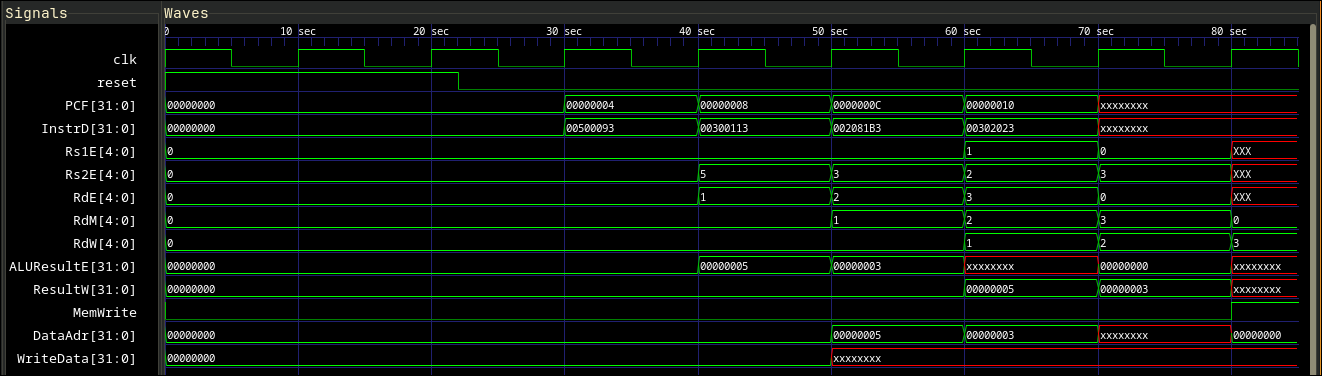
\includegraphics[width=\textwidth]{hazard_forward_nohu.png}
	\caption{Programa de \textit{forward} sin unidad de riesgos: \texttt{ALUResultE}
		queda en \texttt{X} durante el \texttt{add} porque \texttt{x1}/\texttt{x2} aún
		no se han escrito en el banco de registros.}
	\label{fig:hazard-forward-fail}
\end{figure}

\paragraph{Caso \textit{stall}.} La Figura~\ref{fig:hazard-stall-fail} muestra el
riesgo \textit{load-use}: \texttt{add x3,x2,x2} se ejecuta \textbf{inmediatamente
	después} de \texttt{lw x2,8(x0)}, sin darle tiempo a la etapa Memory de traer el
dato. Sin \textit{stall} que detenga un ciclo al \texttt{add}, este lee el valor
\textbf{viejo} de \texttt{x2} (el que había antes del \texttt{lw}) en vez del
recién cargado. El resultado se ve al final de la traza: \texttt{WriteData} llega
en \texttt{xxxxxxxx} a la escritura final, en vez del \texttt{14} esperado.

\begin{figure}[H]
	\centering
	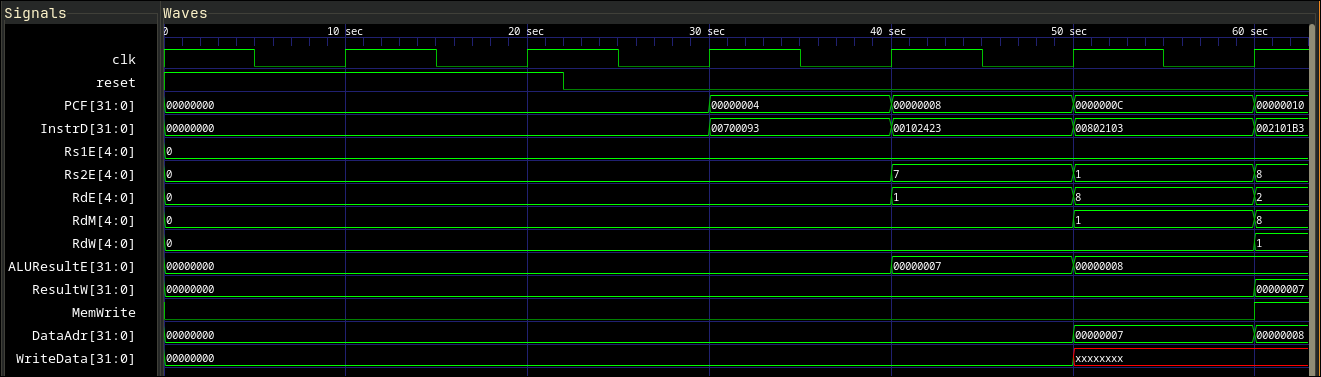
\includegraphics[width=\textwidth]{hazard_stall_nohu.png}
	\caption{Programa de \textit{stall} sin unidad de riesgos: el \texttt{add}
		inmediatamente posterior al \texttt{lw} no espera el dato de memoria;
		\texttt{WriteData} termina indefinido.}
	\label{fig:hazard-stall-fail}
\end{figure}

\paragraph{Caso \textit{flush}.} La Figura~\ref{fig:hazard-flush-fail} muestra el
riesgo de control: el \texttt{beq x1,x0,SKIP} se toma (\texttt{x1=0}), pero sin
\textit{flush} las dos instrucciones del camino secuencial equivocado
(\texttt{addi x2,x0,99} y \texttt{sw x2,0(x0)}), ya captadas antes de resolver el
salto, \textbf{se ejecutan igual}. Se observa \texttt{ALUResultE = 0x63} (99 en
decimal) y, poco después, una escritura a \texttt{DataAdr = 0} con ese valor: el
camino erróneo alcanza a escribir en memoria antes de que el programa continúe
por \texttt{SKIP}, violando la condición de la prueba (``la única escritura debe
ser \texttt{Mem[4]=5}'').

\begin{figure}[H]
	\centering
	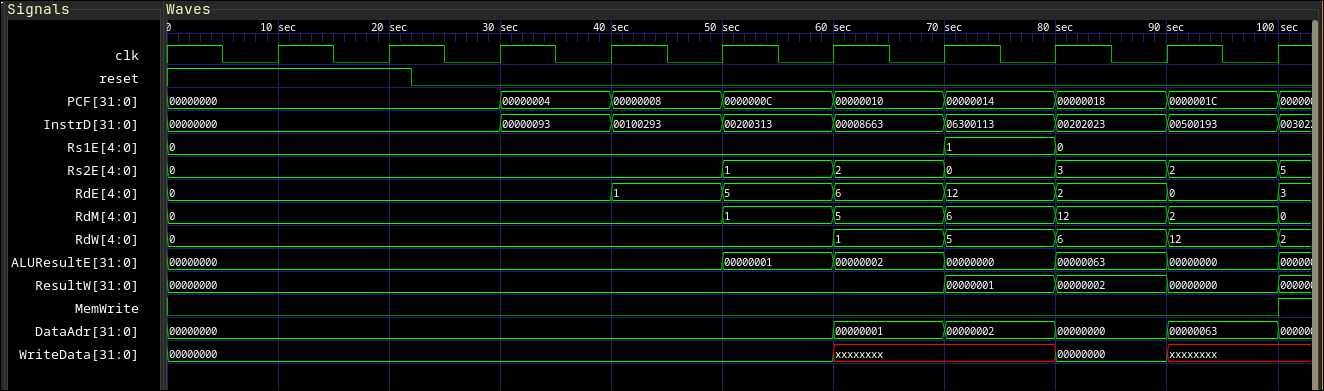
\includegraphics[width=\textwidth]{hazard_flush_nohu.png}
	\caption{Programa de \textit{flush} sin unidad de riesgos: las instrucciones del
		camino erróneo tras el \texttt{beq} tomado no se descartan y llegan a escribir
		\texttt{Mem[0]=99} (\texttt{0x63}).}
	\label{fig:hazard-flush-fail}
\end{figure}

En los tres casos la causa es la misma: el pipeline base no tiene forma de
detectar ni corregir estas situaciones por sí solo, y necesita la unidad de
riesgos (Sección~\ref{sec:hazard-unit-impl}) para resolverlas.

\subsection{Implementación de la Hazard Unit}
\label{sec:hazard-unit-impl}

La implementación siguió la organización mostrada en la arquitectura objetivo del
pipeline: una \textbf{hazard unit separada} del \textit{datapath} y de la unidad de
control, encargada de generar las señales de adelantamiento, detención y descarte. La
idea fue mantener la detección de riesgos en un único bloque y propagar sus decisiones al
resto del procesador con el menor número posible de cambios estructurales.

\subsubsection{Módulo \texttt{hazardunit.v}}

Se creó el módulo \texttt{hazardunit.v}, que compara los registros fuente de Decode y
Execute con los registros destino presentes en Execute, Memory y Writeback. A partir de
esas comparaciones produce seis salidas: \texttt{ForwardAE}, \texttt{ForwardBE},
\texttt{StallF}, \texttt{StallD}, \texttt{FlushD} y \texttt{FlushE}.

\begin{lstlisting}
assign lwStall = (ResultSrcE == 2'b01) &
                 ((Rs1D != 0 && Rs1D == RdE) ||
                  (Rs2D != 0 && Rs2D == RdE));

assign ForwardAE = (Rs1E != 0 && Rs1E == RdM && RegWriteM) ? 2'b10 :
                   (Rs1E != 0 && Rs1E == RdW && RegWriteW) ? 2'b01 : 2'b00;

assign ForwardBE = (Rs2E != 0 && Rs2E == RdM && RegWriteM) ? 2'b10 :
                   (Rs2E != 0 && Rs2E == RdW && RegWriteW) ? 2'b01 : 2'b00;
\end{lstlisting}

Las señales de la unidad tienen el siguiente papel:

\begin{itemize}
	\item \textbf{\texttt{ForwardAE}/\texttt{ForwardBE}:} seleccionan, para cada operando
	      de Execute, si se usa el valor leído desde el banco de registros
	      (\texttt{00}), el valor reenviado desde Writeback (\texttt{01}) o el valor
	      reenviado desde Memory (\texttt{10}).
	\item \textbf{\texttt{StallF}/\texttt{StallD}:} congelan Fetch y Decode cuando se
	      detecta un caso \textit{load-use}; así se evita que la instrucción dependiente
	      avance antes de que el dato cargado esté disponible.
	\item \textbf{\texttt{FlushD}/\texttt{FlushE}:} anulan instrucciones ya captadas.
	      \texttt{FlushD} descarta la instrucción incorrecta en IF/ID tras un salto tomado,
	      mientras que \texttt{FlushE} inserta una burbuja en ID/EX tanto para \textit{load-use}
	      como para cambios de flujo de control.
\end{itemize}

\subsubsection{Nuevos registros de pipeline con control}

El diseño original utilizaba únicamente \texttt{flopr}, que solo permitía reloj y reset.
Eso no era suficiente para una hazard unit, porque para detener o descartar instrucciones
se necesita distinguir entre \textbf{mantener el valor actual} y \textbf{limpiarlo a
	cero}. Por eso se añadieron dos bloques auxiliares:

\begin{itemize}
	\item \texttt{flopenr.v}: registro con \textit{enable}, usado cuando una etapa debe
	      poder \textbf{congelarse}.
	\item \texttt{flopenrc.v}: registro con \textit{enable} y \textit{clear}, usado cuando
	      además de congelar una etapa se necesita \textbf{inyectar una burbuja}.
\end{itemize}

\begin{lstlisting}
always @(posedge clk or posedge reset) begin
  if (reset) q <= 0;
  else if (clear) q <= 0;
  else if (en) q <= d;
end
\end{lstlisting}

\subsubsection{Cambios en \texttt{datapath.v}}

El \textit{datapath} recibió la mayor parte de la integración física de la unidad de
riesgos. Los cambios principales fueron tres.

Primero, el registro del PC pasó a usar \texttt{flopenr}, y los registros IF/ID pasaron
a usar \texttt{flopenrc}. Esto permite congelar Fetch y Decode con
\texttt{StallF}/\texttt{StallD} y descartar la instrucción de Decode con
\texttt{FlushD}.

\begin{lstlisting}
flopenr #(WIDTH) pcreg(... .en(~StallF), .d(PCNextF), .q(PCF));
flopenrc #(WIDTH) ifid_instrreg(... .en(~StallD), .clear(FlushD), ...);
\end{lstlisting}

Segundo, los registros ID/EX también se cambiaron a \texttt{flopenrc}. Esto permite que
\texttt{FlushE} convierta el contenido de Execute en una burbuja cuando hay un salto
tomado o un \textit{load-use}.

Tercero, se añadieron multiplexores de forwarding delante de la ALU. El operando A se
selecciona con \texttt{ForwardAE}; el operando B se selecciona con
\texttt{ForwardBE} antes del multiplexor de inmediato. Además, el mismo valor adelantado
de B se reutiliza como \texttt{WriteDataE}, de modo que el \texttt{store} también recibe
el dato correcto cuando depende de una instrucción anterior.

\begin{lstlisting}
mux3 #(WIDTH) forwardamux(... .s(ForwardAE), .y(SrcAE));
mux3 #(WIDTH) forwardbmux(... .s(ForwardBE), .y(WriteDataE));
mux2 #(WIDTH) srcbmux(.d0(WriteDataE), .d1(ImmExtE), .s(ALUSrcE), .y(SrcBE));
\end{lstlisting}

Finalmente, se creó un \texttt{ResultM} interno en Memory. Esto permite reenviar no solo
el resultado de ALU, sino el resultado \textbf{real} de la instrucción que está en M,
siguiendo la selección marcada por \texttt{ResultSrcM}.

\subsubsection{Cambios en \texttt{controller.v}}

En la unidad de control no se añadió la detección de riesgos; esa lógica quedó en
\texttt{hazardunit.v}. El cambio aquí fue permitir que la tubería de control en Execute
también pueda vaciarse cuando la hazard unit lo ordene. Para eso, los registros
\texttt{regE} y \texttt{funct3Ereg} dejaron de ser \texttt{flopr} y pasaron a ser
\texttt{flopenrc}, gobernados por \texttt{FlushE}.

\begin{lstlisting}
flopenrc #(12) regE(... .en(1'b1), .clear(FlushE), .d(controlsE_in), .q(controlsE));
flopenrc #(3)  funct3Ereg(... .en(1'b1), .clear(FlushE), .d(funct3D), .q(funct3E));
\end{lstlisting}

Esto es importante porque una burbuja no debe limpiar solo los \textbf{datos} de ID/EX,
sino también las \textbf{señales de control}. Si no se hiciera así, una instrucción ya
descartada podría seguir produciendo una escritura en memoria o un cambio de flujo.

\subsubsection{Cambios en \texttt{riscvpipe.v}}

El módulo \texttt{riscvpipe.v} se convirtió en el punto de interconexión entre control,
datapath y hazard unit. Aquí se añadieron las nuevas señales intermedias:

\begin{itemize}
	\item registros fuente y destino por etapa:
	      \texttt{Rs1D}, \texttt{Rs2D}, \texttt{Rs1E}, \texttt{Rs2E}, \texttt{RdE},
	      \texttt{RdM}, \texttt{RdW};
	\item señales de control para hazards:
	      \texttt{ForwardAE}, \texttt{ForwardBE}, \texttt{StallF}, \texttt{StallD},
	      \texttt{FlushD}, \texttt{FlushE};
	\item señales intermedias para decidir el forwarding:
	      \texttt{ResultSrcE}, \texttt{ResultSrcM} y \texttt{RegWriteM}.
\end{itemize}

Con estas conexiones, \texttt{riscvpipe} ya no solo instancia \texttt{controller} y
\texttt{datapath}, sino que añade un tercer bloque especializado, \texttt{hazardunit},
que observa el estado de la tubería y decide cómo resolver dinámicamente cada riesgo.

\subsubsection{Resultado estructural}

Tras estos cambios, la arquitectura final coincide con la organización esperada del
pipeline con hazard unit: el \textit{datapath} sigue transportando datos, la unidad de
control sigue generando señales funcionales, y la \textbf{hazard unit} se encarga de
supervisar dependencias y cambios de flujo para generar \texttt{forward}, \texttt{stall}
y \texttt{flush}. Esto completa la transición desde un pipeline base que dependía de
\texttt{NOP} manuales hacia un pipeline que resuelve los riesgos de forma automática.

La Figura~\ref{fig:hazard-demo} muestra la ejecución del \textit{script}
\texttt{run\_hazard\_demo.sh} una vez incorporada la hazard unit. En ella se verifica que
los tres casos de prueba asociados a \textit{forwarding}, \textit{stalling} y
\textit{flushing} pasan correctamente, confirmando que la resolución automática de
riesgos ya funciona en el procesador final.

\begin{figure}[H]
	\centering
	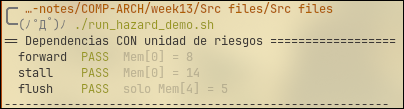
\includegraphics[width=0.8\textwidth]{hazard_demo.png}
	\caption{Salida de \texttt{run\_hazard\_demo.sh} tras implementar la hazard unit:
		los casos de \textit{forward}, \textit{stall} y \textit{flush} pasan correctamente.}
	\label{fig:hazard-demo}
\end{figure}

\subsection{Programas de prueba}

Además de la salida resumida del \textit{script} de pruebas, se analizaron los
\textit{waveforms} de los programas de hazard para observar directamente la acción de la
unidad de riesgos dentro del pipeline. En los apartados siguientes se estudian por
separado los tres mecanismos implementados: \textit{forward}, \textit{stall} y
\textit{flush}.

\subsubsection{Caso \textit{forward}}

La Figura~\ref{fig:hazard-forward-wave} muestra la simulación del caso de
\textit{forwarding}.

\begin{figure}[H]
	\centering
	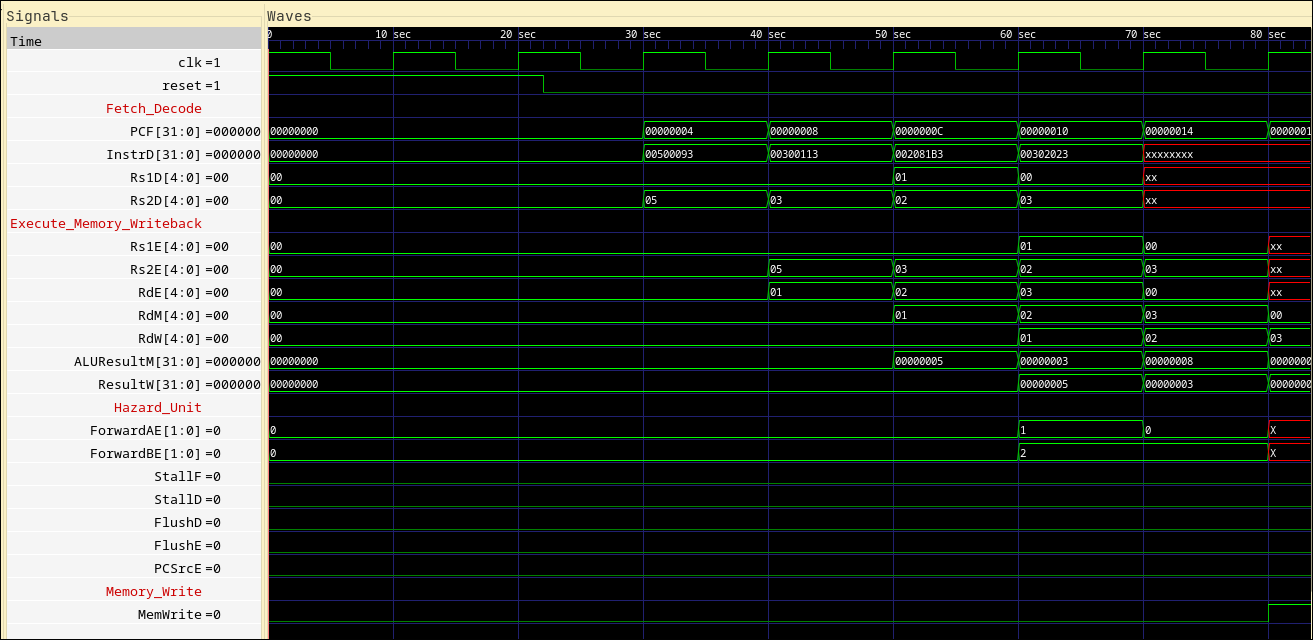
\includegraphics[width=\textwidth]{hazard_forward_waveform.png}
	\caption{Waveform del programa de prueba de \textit{forwarding}.}
	\label{fig:hazard-forward-wave}
\end{figure}

En esta captura se observan varios comportamientos importantes. Primero, \texttt{PCF} y
\texttt{InstrD} muestran el avance normal del programa por Fetch y Decode. Segundo, los
registros destino avanzan por la tubería a través de \texttt{RdE}, \texttt{RdM} y
\texttt{RdW}, confirmando que las instrucciones se encuentran simultáneamente en varias
etapas.

El punto clave es la activación de \texttt{ForwardAE} y \texttt{ForwardBE}. Estas señales
indican que la instrucción \texttt{add x3, x1, x2} no toma sus operandos desde el banco de
registros, sino que recibe datos reenviados desde etapas posteriores del pipeline. Al
mismo tiempo, \texttt{StallF}, \texttt{StallD}, \texttt{FlushD} y \texttt{FlushE}
permanecen en cero, lo que confirma que este riesgo se resuelve únicamente con
\textit{forwarding}, sin detener ni vaciar el pipeline.

Finalmente, la activación de \texttt{MemWrite} al final de la ejecución muestra que el
resultado correcto llega a memoria una vez resuelta la dependencia. Por tanto, el
waveform confirma visualmente que la hazard unit soluciona el riesgo RAW del programa de
prueba exactamente de la forma esperada por la teoría.

\subsubsection{Caso \textit{stall}}

La Figura~\ref{fig:hazard-stall-wave} muestra ahora el caso \textit{load-use}, donde el
adelantamiento por sí solo no basta y la hazard unit debe introducir una detención de un
ciclo.

\begin{figure}[H]
	\centering
	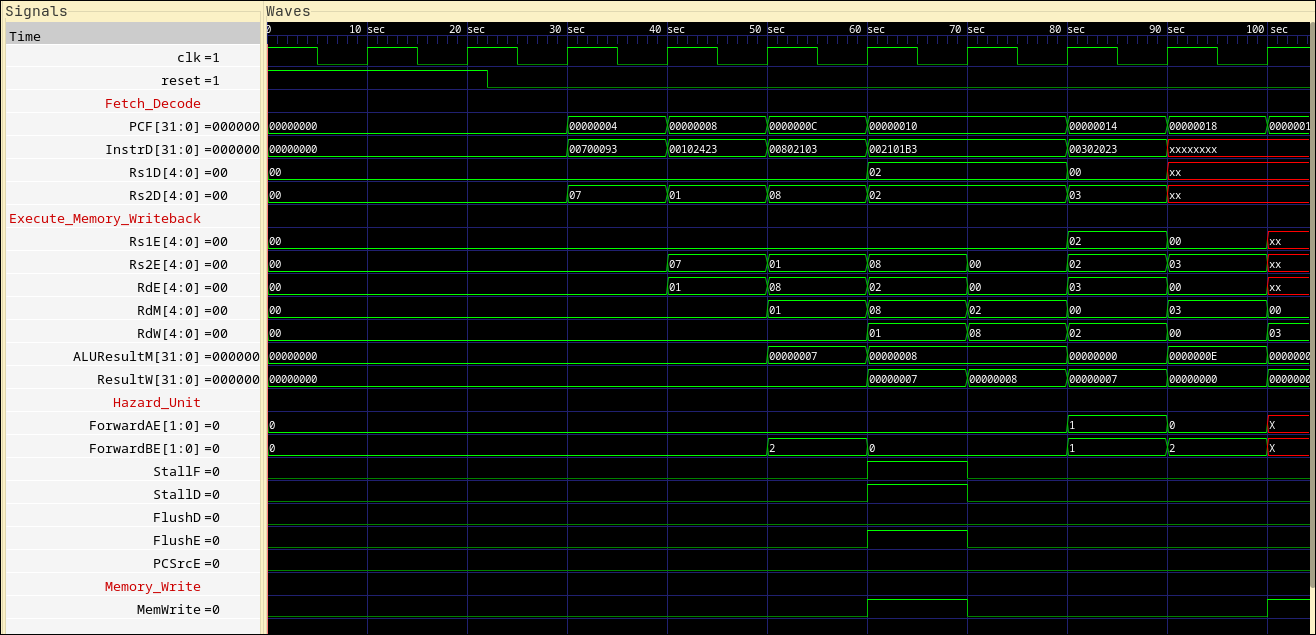
\includegraphics[width=\textwidth]{hazard_stall_waveform.png}
	\caption{Waveform del programa de prueba de \textit{stall}.}
	\label{fig:hazard-stall-wave}
\end{figure}

En esta captura se observa primero el flujo normal del programa por \texttt{PCF} y
\texttt{InstrD}: la secuencia corresponde a \texttt{addi}, \texttt{sw}, \texttt{lw},
\texttt{add} y \texttt{sw}. El conflicto aparece cuando la instrucción
\texttt{add x3, x2, x2} intenta usar inmediatamente el valor producido por
\texttt{lw x2, 8(x0)}.

La evidencia directa del mecanismo es la activación simultánea de \texttt{StallF} y
\texttt{StallD}, junto con \texttt{FlushE}. Esto significa que la hazard unit congela
Fetch y Decode durante un ciclo e inserta una burbuja en Execute, exactamente como exige
el tratamiento de un riesgo \textit{load-use}. Al mismo tiempo, \texttt{FlushD} y
\texttt{PCSrcE} permanecen en cero, lo que confirma que no se trata de un salto ni de un
descarte por control, sino exclusivamente de una detención por dependencia de datos.

Después de ese ciclo de espera, el pipeline reanuda su avance normal y aparecen nuevas
activaciones de \texttt{ForwardAE} y \texttt{ForwardBE}, indicando que el dato ya puede
completarse mediante forwarding en las etapas siguientes. Finalmente,
\texttt{ALUResultM} muestra el valor \texttt{14} y \texttt{MemWrite} confirma su
escritura correcta en memoria. Por tanto, este waveform muestra que la hazard unit no
solo detecta el conflicto \textit{load-use}, sino que lo resuelve correctamente mediante
la combinación de \textit{stall} y forwarding.

\subsubsection{Caso \textit{flush}}

La Figura~\ref{fig:hazard-flush-wave} muestra el caso de riesgo de control. El programa
ejecuta un \texttt{beq x1, x0, SKIP} que resulta tomado, por lo que las instrucciones
captadas inmediatamente después pertenecen al camino secuencial erróneo y deben ser
descartadas.

\begin{figure}[H]
	\centering
	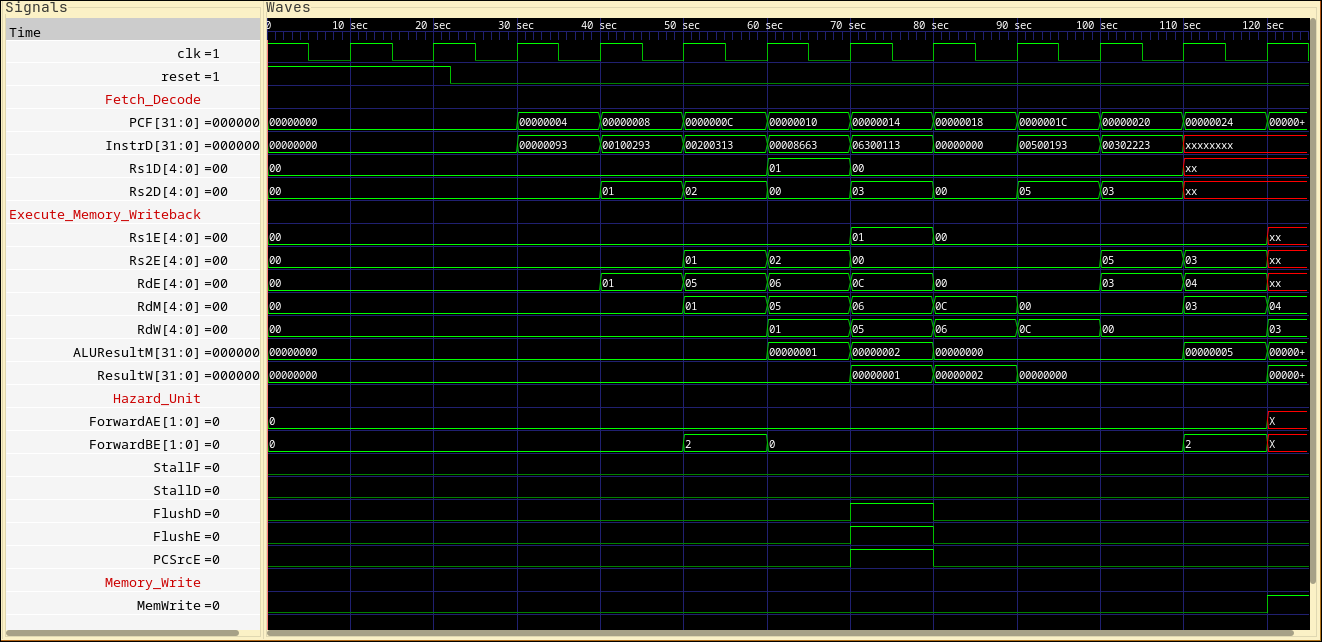
\includegraphics[width=\textwidth]{hazard_flush_waveform.png}
	\caption{Waveform del programa de prueba de \textit{flush}.}
	\label{fig:hazard-flush-wave}
\end{figure}

En la captura se ve primero el flujo normal por \texttt{PCF} e \texttt{InstrD}: aparecen
las instrucciones de inicialización, luego el \texttt{beq} y, a continuación, la
instrucción del camino incorrecto \texttt{06300113} (el \texttt{addi x2, x0, 99}). Justo
después de resolverse el salto, se activan simultáneamente \texttt{PCSrcE},
\texttt{FlushD} y \texttt{FlushE}, mientras que \texttt{StallF} y \texttt{StallD}
permanecen en cero. Esa combinación muestra exactamente el comportamiento esperado para
un hazard de control: no se detiene el pipeline, sino que se \textbf{descartan} las
instrucciones incorrectas ya captadas.

El efecto del descarte también se observa en \texttt{InstrD}, donde tras la activación de
\texttt{PCSrcE} aparece una burbuja (\texttt{00000000}) antes de reanudarse la ejecución
por el camino correcto con \texttt{00500193} y \texttt{00302223}. Más adelante,
\texttt{ALUResultM} muestra el valor \texttt{5} y \texttt{MemWrite} confirma la
escritura final correcta, correspondiente a \texttt{Mem[4] = 5}. No aparece ninguna
escritura errónea asociada al camino descartado, lo que confirma que la hazard unit
resuelve correctamente el riesgo de control mediante \textit{flush}.

En conjunto, los tres programas de prueba muestran que la hazard unit resuelve
correctamente riesgos de datos por \textit{forwarding}, riesgos \textit{load-use} por
\textit{stalling} y riesgos de control por \textit{flushing}.

\subsection{Cómo la hazard unit resuelve las dependencias}

Los tres waveforms permiten ver que la hazard unit no aplica una única estrategia para
todos los conflictos, sino que selecciona el mecanismo adecuado según el tipo de
dependencia detectada:

\begin{itemize}
	\item En el programa de \textit{forward}, la dependencia RAW entre instrucciones
	      consecutivas se resuelve reenviando operandos con \texttt{ForwardAE} y
	      \texttt{ForwardBE}; el pipeline \textbf{no se detiene} y el resultado correcto
	      llega a memoria.
	\item En el programa de \textit{stall}, la dependencia \textit{load-use} no puede
	      resolverse solo con adelantamiento porque el dato de \texttt{lw} todavía no está
	      disponible. La hazard unit entonces activa \texttt{StallF}, \texttt{StallD} y
	      \texttt{FlushE}, inserta una burbuja y después permite completar la operación con
	      el dato correcto.
	\item En el programa de \textit{flush}, el problema no es un dato faltante sino un
	      cambio de flujo. Cuando el \texttt{beq} resulta tomado, la hazard unit activa
	      \texttt{PCSrcE}, \texttt{FlushD} y \texttt{FlushE} para descartar las
	      instrucciones del camino erróneo antes de que modifiquen la memoria o los
	      registros.
\end{itemize}

Por tanto, la evidencia experimental confirma exactamente la función esperada de la
hazard unit: \textbf{adelantar} cuando el dato ya existe en una etapa posterior,
\textbf{detener} cuando el dato aún no puede adelantarse y \textbf{descartar} cuando el
camino de ejecución correcto cambia por un salto. Así, los programas de prueba que antes
fallaban sin \texttt{NOP} manuales pasan ahora correctamente sobre el pipeline final.

\part{Extensión C: instrucciones comprimidas (RVC)}

\section{Introducción a la extensión C}

La extensión \textbf{C} (\textit{compressed}, \textbf{RVC}) de RISC-V define
instrucciones de \textbf{16 bits} que coexisten con las de 32 bits del ISA base,
reduciendo el tamaño del código tipicamente entre un 25\,\% y un 30\,\% sin perder
expresividad. No es un modo aparte que deba activarse: se pueden \textbf{mezclar}
libremente instrucciones de 16 y 32 bits en el mismo flujo de ejecucion.

La propiedad que hace manejable la implementacion es que \textbf{cada instruccion
comprimida tiene exactamente un equivalente de 32 bits}. Por eso la estrategia
elegida es \textbf{descomprimir en la etapa de Fetch}: expandir los 16 bits a su
forma RV32I \emph{antes} del registro de pipeline IF/ID. Asi, las etapas Decode,
Execute, Memory y Writeback, junto con \texttt{controller}, \texttt{aludec},
\texttt{extend} y la unidad de riesgos, \textbf{no se modifican}: el pipeline
interno solo ve instrucciones RV32I normales.

La distincion entre 16 y 32 bits se realiza con los dos bits menos significativos
de la instruccion leida: si \texttt{instr[1:0] != 2'b11}, la instruccion es
comprimida y debe expandirse; en caso contrario es una instruccion estandar de 32
bits.

Esta primera parte de RVC implementa 11 instrucciones aritmeticas y de
registro-inmediato:
\begin{center}
\texttt{c.addi \ c.lui \ c.slli \ c.add \ c.sub \ c.xor \ c.or \ c.and \ c.srli \ c.srai \ c.andi}
\end{center}

\section{Cambios en el datapath para soportar RVC}

Toda la logica nueva se concentra en la etapa de Fetch, en tres cambios. Los
modulos \texttt{controller}, \texttt{aludec}, \texttt{extend},
\texttt{hazardunit}, \texttt{regfile}, \texttt{alu} y \texttt{dmem} no se
modificaron.

\subsection{Memoria de instrucciones con ventana deslizante}

Con instrucciones de 16 bits, el PC puede caer en una direccion par que no es
multiplo de 4 (\texttt{PC[1]=1}), y una instruccion de 32 bits puede quedar
\textbf{partida entre dos palabras} de memoria. La \texttt{imem} deja de devolver
``la palabra alineada'' y pasa a devolver ``los 32 bits que empiezan en el PC'',
ensamblando dos palabras consecutivas cuando hace falta:

\begin{lstlisting}
  wire [31:0] w0, w1;
  assign w0 = RAM[a[31:2]];
  assign w1 = RAM[a[31:2] + 1];
  assign rd = a[1] ? {w1[15:0], w0[31:16]} : w0;
\end{lstlisting}

Para programas RV32I puros, \texttt{PC[1]=0} siempre, de modo que
\texttt{rd = RAM[k]} y el comportamiento es identico al original.

\subsection{Incremento variable del PC (\texttt{+2/+4})}

El incremento fijo \texttt{PC+4} se reemplaza por uno que depende del tamano de la
instruccion leida (2 bytes si es comprimida, 4 si es normal):

\begin{lstlisting}
  assign PCPlusIncF = PCF + (compressedF ? 32'd2 : 32'd4);
\end{lstlisting}

La senal \texttt{compressedF} la produce el descompresor en el mismo ciclo de
Fetch. Se renombro \texttt{PCPlus4} a \texttt{PCPlusInc} en toda la tuberia, ya
que ese valor es ademas la direccion de retorno de \texttt{jal}/\texttt{jalr}.

\subsection{Modulo descompresor}

Es un modulo combinacional nuevo (\texttt{decompressor.v}), cableado sobre la
instruccion cruda en Fetch. Calcula la senal \texttt{compressed} (que maneja el
\texttt{+2/+4}) y produce la instruccion de 32 bits ya expandida, que es la que se
guarda en el registro IF/ID:

\begin{lstlisting}
  decompressor dec(
    .instrraw(InstrF),
    .instr(InstrDecF),
    .compressed(compressedF)
  );
\end{lstlisting}

El registro IF/ID guarda \texttt{InstrDecF} (la instruccion expandida), no la
cruda. De esa forma, todo lo que esta aguas abajo recibe una instruccion RV32I
normal.

\section{Implementacion de las instrucciones comprimidas}

Las 11 instrucciones comparten una misma forma: \texttt{rd = rd op algo} (el
registro destino es tambien el primer operando; por eso RVC ahorra bits). El
descompresor las decodifica con un \texttt{case} sobre \texttt{\{op, funct3\}} y,
donde hace falta, sub-campos adicionales. Los registros restringidos
\texttt{rd'/rs2'} de los formatos CA y CB se mapean al rango x8--x15 anteponiendo
\texttt{01} a sus 3 bits:

\begin{lstlisting}
  wire [4:0] rdp  = {2'b01, c[9:7]};
  wire [4:0] rs2p = {2'b01, c[4:2]};
\end{lstlisting}

\subsection{Formato CI: \texttt{c.addi}, \texttt{c.lui}, \texttt{c.slli}}

Usan un registro completo (5 bits) y un inmediato de 6 bits formado por
\texttt{\{c[12], c[6:2]\}}.

\begin{lstlisting}
  5'b01_000: instr = {immci, rd, 3'b000, rd, 7'b0010011};   // c.addi -> addi rd,rd,imm
  5'b01_011: instr = {immlui, rd, 7'b0110111};              // c.lui  -> lui rd,imm
  5'b10_000: instr = {7'b0000000, shamt, rd, 3'b001, rd, 7'b0010011}; // c.slli
\end{lstlisting}

\begin{itemize}[noitemsep]
  \item \texttt{c.addi}: el inmediato \texttt{immci = \{\{7\{c[12]\}\}, c[6:2]\}}
        es la extension de signo de 6 a 12 bits.
  \item \texttt{c.lui}: \texttt{immlui = \{\{15\{c[12]\}\}, c[6:2]\}} ocupa
        imm[31:12]; el destino no puede ser x0 ni x2.
  \item \texttt{c.slli}: el shamt son los 5 bits \texttt{c[6:2]}; funct7=0000000,
        funct3=001.
\end{itemize}

\subsection{Formato CR: \texttt{c.add}}

Usa dos registros completos. Comparte \texttt{\{op,funct3\}=\{10,100\}} con otras
instrucciones del cuadrante 2, asi que se distingue por \texttt{c[12]=1} y
\texttt{rs2 != 0}:

\begin{lstlisting}
  5'b10_100: instr = (c[12] && rs2 != 0)
                   ? {7'b0000000, rs2, rd, 3'b000, rd, 7'b0110011}  // c.add -> add rd,rd,rs2
                   : instrraw;
\end{lstlisting}

\subsection{Formato CA: \texttt{c.sub}, \texttt{c.xor}, \texttt{c.or}, \texttt{c.and}}

Operaciones registro-registro con registros restringidos x8--x15. Comparten
\texttt{\{op,funct3\}=\{01,100\}}; dentro, \texttt{c[11:10]=11} indica la familia
CA y \texttt{c[6:5]} elige la operacion:

\begin{lstlisting}
  2'b11: case (c[6:5])
           2'b00: instr = {7'b0100000, rs2p, rdp, 3'b000, rdp, 7'b0110011}; // c.sub
           2'b01: instr = {7'b0000000, rs2p, rdp, 3'b100, rdp, 7'b0110011}; // c.xor
           2'b10: instr = {7'b0000000, rs2p, rdp, 3'b110, rdp, 7'b0110011}; // c.or
           2'b11: instr = {7'b0000000, rs2p, rdp, 3'b111, rdp, 7'b0110011}; // c.and
         endcase
\end{lstlisting}

Solo \texttt{c.sub} usa funct7=0100000; las demas, 0000000. El funct3 distingue la
operacion logica.

\subsection{Formato CB: \texttt{c.srli}, \texttt{c.srai}, \texttt{c.andi}}

Un registro restringido y un inmediato/shamt de 6 bits. Comparten la misma entrada
\texttt{\{01,100\}}; se distinguen por \texttt{c[11:10]}:

\begin{lstlisting}
  2'b00: instr = {7'b0000000, shamt, rdp, 3'b101, rdp, 7'b0010011}; // c.srli
  2'b01: instr = {7'b0100000, shamt, rdp, 3'b101, rdp, 7'b0010011}; // c.srai
  2'b10: instr = {immci, rdp, 3'b111, rdp, 7'b0010011};             // c.andi
\end{lstlisting}

\texttt{c.srli} y \texttt{c.srai} se diferencian por funct7 (logico vs
aritmetico); \texttt{c.andi} reusa el inmediato con signo \texttt{immci}.

\section{Instrucciones de memoria y control de flujo (Parte 2 de RVC)}

Esta segunda tanda anade las 10 instrucciones restantes: acceso a memoria
(\texttt{c.lw}, \texttt{c.sw}, \texttt{c.lwsp}, \texttt{c.swsp}) y control de
flujo (\texttt{c.beqz}, \texttt{c.bnez}, \texttt{c.j}, \texttt{c.jal},
\texttt{c.jr}, \texttt{c.jalr}). La estrategia sigue siendo
\textbf{descomprimir en Fetch}: ninguna toca las etapas posteriores.

La novedad principal es que cada formato trae su propio \emph{inmediato
barajado} (\textit{scrambled}): los bits del \textit{offset} no estan
contiguos en la instruccion de 16 bits, sino repartidos para maximizar la
densidad. Se declaran como \textit{wires} con nombre para hacerlos legibles:

\begin{lstlisting}
  wire [6:0]  offlw  = {c[5], c[12:10], c[6], 2'b00};      // CL/CS (c.lw/c.sw)
  wire [7:0]  offsp  = {c[3:2], c[12], c[6:4], 2'b00};     // c.lwsp
  wire [7:0]  offssp = {c[8:7], c[12:9], 2'b00};           // c.swsp
  wire [8:0]  offcb  = {c[12], c[6:5], c[2],
                        c[11:10], c[4:3], 1'b0};            // c.beqz/c.bnez
  wire [11:0] offcj  = {c[12], c[8], c[10], c[9], c[6],
                        c[7], c[2], c[11], c[5:3], 1'b0};   // c.j/c.jal
\end{lstlisting}

\subsection{Memoria con registros restringidos: \texttt{c.lw}, \texttt{c.sw}}

Formatos CL y CS: registros restringidos \texttt{x8}--\texttt{x15} y un
\textit{offset} de 5 bits alineado a palabra. \texttt{c.lw} expande a un
\texttt{lw} tipo~I; \texttt{c.sw} a un \texttt{sw} tipo~S (con el inmediato
partido en \texttt{imm[11:5]} e \texttt{imm[4:0]}):

\begin{lstlisting}
  5'b00_010: instr = {5'b0, offlw, rs1p, 3'b010, rs2p, 7'b0000011};   // c.lw
  5'b00_110: instr = {5'b0, offlw[6:5], rs2p, rs1p, 3'b010,
                       offlw[4:2], 2'b00, 7'b0100011};                // c.sw
\end{lstlisting}

Un detalle facil de confundir: el registro destino de \texttt{c.lw}
(\texttt{rd'}) vive en \texttt{c[4:2]} (la misma posicion que \texttt{rs2'} en
CS), \textbf{no} en \texttt{c[9:7]}. Por eso se reutiliza \texttt{rs2p} como
destino.

\subsection{Memoria relativa a la pila: \texttt{c.lwsp}, \texttt{c.swsp}}

Formatos CI y CSS: la base es siempre \texttt{x2} (\textit{stack pointer}) y el
registro puede ser cualquiera de los 32. Cada uno baraja el \textit{offset}
distinto:

\begin{lstlisting}
  5'b10_010: instr = {4'b0, offsp, 5'b00010, 3'b010, rd, 7'b0000011};  // c.lwsp
  5'b10_110: instr = {4'b0, offssp[7:5], rs2, 5'b00010, 3'b010,
                       offssp[4:0], 7'b0100011};                       // c.swsp
\end{lstlisting}

\subsection{Branches condicionales: \texttt{c.beqz}, \texttt{c.bnez}}

Formato CB: comparan un registro restringido contra \texttt{x0} (de ahi el
sufijo \textit{-z}, ``zero''). Expanden a \texttt{beq}/\texttt{bne} con
\texttt{rs2 = x0} y el \textit{offset} de 8 bits reordenado al formato~B:

\begin{lstlisting}
  5'b01_110: instr = {offcb[8], {3{offcb[8]}}, offcb[7:5], 5'b00000,
                       rs1p, 3'b000, offcb[4:1], offcb[8], 7'b1100011}; // c.beqz
  5'b01_111: instr = {offcb[8], {3{offcb[8]}}, offcb[7:5], 5'b00000,
                       rs1p, 3'b001, offcb[4:1], offcb[8], 7'b1100011}; // c.bnez
\end{lstlisting}

\subsection{Saltos incondicionales: \texttt{c.j}, \texttt{c.jal}}

Formato CJ: \textit{offset} de 11 bits. \texttt{c.j} expande a \texttt{jal x0}
(descarta la direccion de retorno) y \texttt{c.jal} a \texttt{jal x1} (la
guarda). El \textit{offset} se reordena al desperdigado formato~J:

\begin{lstlisting}
  5'b01_101: instr = {offcj[11], offcj[10:1], offcj[11],
                       {8{offcj[11]}}, 5'b00000, 7'b1101111};  // c.j  -> jal x0
  5'b01_001: instr = {offcj[11], offcj[10:1], offcj[11],
                       {8{offcj[11]}}, 5'b00001, 7'b1101111};  // c.jal -> jal x1
\end{lstlisting}

\subsection{Saltos a registro: \texttt{c.jr}, \texttt{c.jalr}}

Formato CR. Comparten \texttt{\{op,funct3\}=\{10,100\}} con \texttt{c.mv} y
\texttt{c.add} (de la Parte~1). La desambiguacion usa \texttt{c[12]} y si
\texttt{rs2} es cero:

\begin{lstlisting}
  5'b10_100:
    if (!c[12] && rs2 == 5'b0)
      instr = {12'b0, rd, 3'b000, 5'b00000, 7'b1100111}; // c.jr   -> jalr x0
    else if (!c[12])
      instr = {7'b0, rs2, 5'b00000, 3'b000, rd, 7'b0110011}; // c.mv -> add rd,x0,rs2
    else if (rs2 == 5'b0)
      instr = {12'b0, rd, 3'b000, 5'b00001, 7'b1100111}; // c.jalr -> jalr x1
    else
      instr = {7'b0000000, rs2, rd, 3'b000, rd, 7'b0110011}; // c.add
\end{lstlisting}

\texttt{c.jr rs1} salta a \texttt{rs1} sin guardar retorno (\texttt{rd=x0});
\texttt{c.jalr rs1} salta guardando el retorno en \texttt{x1}.

\subsection{Cambios en el datapath}

Al igual que en la Parte~1 de RVC, \textbf{no hubo ningun cambio en el
datapath ni en el resto de modulos}: todas las instrucciones nuevas son casos
adicionales dentro del \texttt{decompressor.v} combinacional. Las de memoria se
expanden a \texttt{lw}/\texttt{sw} que el pipeline ya ejecutaba; las de control
a \texttt{beq}/\texttt{bne}/\texttt{jal}/\texttt{jalr} que la unidad de riesgos
ya resolvia (\textit{flush} en salto tomado). El unico cuidado extra fue
respetar el ``no hay \texttt{auipc}'' del Cuadro~1 al escribir los programas de
prueba.

\subsection{Encoding de todas las instrucciones (Parte 1 y Parte 2)}

El Cuadro~\ref{cuadro:encoding} resume la codificacion de las 21 instrucciones
comprimidas implementadas, con su cuadrante (\texttt{op = c[1:0]}), su
\texttt{funct3 = c[15:13]}, el formato RVC y la instruccion RV32I equivalente a
la que expande el descompresor.

\begin{table}[H]
	\centering
	\small
	\begin{tabular}{@{}llllll@{}}
		\toprule
		\textbf{Instr.} & \textbf{op} & \textbf{funct3} & \textbf{Formato} & \textbf{Expande a} & \textbf{Parte} \\
		\midrule
		\texttt{c.addi} & 01 & 000 & CI  & \texttt{addi rd, rd, imm}       & 1 \\
		\texttt{c.jal}  & 01 & 001 & CJ  & \texttt{jal x1, off}            & 2 \\
		\texttt{c.lui}  & 01 & 011 & CI  & \texttt{lui rd, imm}            & 1 \\
		\texttt{c.srli} & 01 & 100 & CB  & \texttt{srli rd', rd', shamt}   & 1 \\
		\texttt{c.srai} & 01 & 100 & CB  & \texttt{srai rd', rd', shamt}   & 1 \\
		\texttt{c.andi} & 01 & 100 & CB  & \texttt{andi rd', rd', imm}     & 1 \\
		\texttt{c.sub}  & 01 & 100 & CA  & \texttt{sub rd', rd', rs2'}     & 1 \\
		\texttt{c.xor}  & 01 & 100 & CA  & \texttt{xor rd', rd', rs2'}     & 1 \\
		\texttt{c.or}   & 01 & 100 & CA  & \texttt{or rd', rd', rs2'}      & 1 \\
		\texttt{c.and}  & 01 & 100 & CA  & \texttt{and rd', rd', rs2'}     & 1 \\
		\texttt{c.j}    & 01 & 101 & CJ  & \texttt{jal x0, off}            & 2 \\
		\texttt{c.beqz} & 01 & 110 & CB  & \texttt{beq rs1', x0, off}      & 2 \\
		\texttt{c.bnez} & 01 & 111 & CB  & \texttt{bne rs1', x0, off}      & 2 \\
		\texttt{c.slli} & 10 & 000 & CI  & \texttt{slli rd, rd, shamt}     & 1 \\
		\texttt{c.lwsp} & 10 & 010 & CI  & \texttt{lw rd, off(x2)}         & 2 \\
		\texttt{c.jr}   & 10 & 100 & CR  & \texttt{jalr x0, rs1, 0}        & 2 \\
		\texttt{c.mv}$^\dagger$ & 10 & 100 & CR & \texttt{add rd, x0, rs2} & --- \\
		\texttt{c.jalr} & 10 & 100 & CR  & \texttt{jalr x1, rs1, 0}        & 2 \\
		\texttt{c.add}  & 10 & 100 & CR  & \texttt{add rd, rd, rs2}        & 1 \\
		\texttt{c.swsp} & 10 & 110 & CSS & \texttt{sw rs2, off(x2)}        & 2 \\
		\texttt{c.lw}   & 00 & 010 & CL  & \texttt{lw rd', off(rs1')}      & 2 \\
		\texttt{c.sw}   & 00 & 110 & CS  & \texttt{sw rs2', off(rs1')}     & 2 \\
		\bottomrule
	\end{tabular}
	\caption{Codificacion de las instrucciones comprimidas implementadas.
		$^\dagger$\texttt{c.mv} aparecio como subproducto de la desambiguacion del
		cuadrante 2, pero no era objetivo del proyecto.}
	\label{cuadro:encoding}
\end{table}

\section{Resultados}

\subsection{Programa de prueba: multiplicacion sin \texttt{MUL}}

El ISA base RV32I no incluye instruccion de multiplicacion. El programa de prueba
calcula \texttt{6 $\times$ 10} mediante la tecnica de \emph{shift-and-add}:
\[
6 \times 10 = 6 \times 8 + 6 \times 2 = (6 \ll 3) + (6 \ll 1).
\]
Mezcla instrucciones de 32 bits (\texttt{addi}, \texttt{sw}) con comprimidas de 16
bits (\texttt{c.slli}, \texttt{c.add}):

\begin{lstlisting}
    addi x8, x0, 6     ; x8 = 6            (32 bits)
    addi x9, x0, 6     ; copia            (32 bits)
    slli x8, x8, 3     ; c.slli: 6<<3 = 48 (16 bits)
    slli x9, x9, 1     ; c.slli: 6<<1 = 12 (16 bits)
    add  x8, x8, x9    ; c.add:  48+12 = 60 (16 bits)
    sw   x8, 0(x0)     ; Mem[0] = 60       (32 bits)
\end{lstlisting}

El resultado esperado es \texttt{Mem[0] = 60}.

\subsection{Waveform}

La Figura~\ref{fig:mul10wave} muestra la ejecucion completa del programa.

\begin{figure}[H]
  \centering
  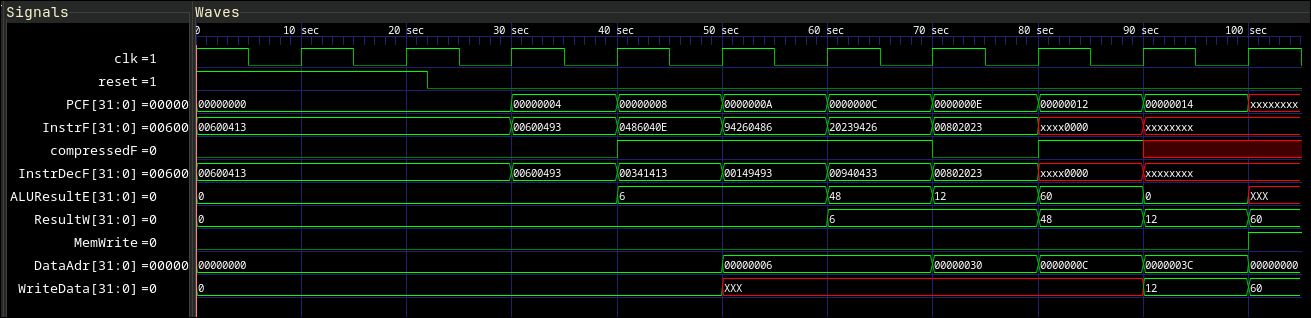
\includegraphics[width=\linewidth]{mul10_waveform.png}
  \caption{Ejecucion de la multiplicacion \texttt{6$\times$10} por
  \emph{shift-and-add}. Se observan el incremento variable del PC, la
  descompresion (\texttt{InstrF} cruda vs \texttt{InstrDecF} expandida) y el
  resultado intermedio de la ALU.}
  \label{fig:mul10wave}
\end{figure}

En el waveform se verifican, paso a paso, los mecanismos implementados:

\begin{itemize}[leftmargin=1.6em]
  \item \textbf{Incremento variable del PC.} \texttt{PCF} avanza \texttt{+4} en las
        instrucciones de 32 bits (\texttt{0x0}$\to$\texttt{0x4}$\to$\texttt{0x8})
        y \texttt{+2} en las comprimidas
        (\texttt{0x8}$\to$\texttt{0xA}$\to$\texttt{0xC}$\to$\texttt{0xE}).
  \item \textbf{Deteccion de comprimida.} \texttt{compressedF} sube a 1 justo
        durante las tres instrucciones de 16 bits.
  \item \textbf{Descompresion.} Comparando \texttt{InstrF} (cruda) con
        \texttt{InstrDecF} (expandida): la comprimida \texttt{0x040E} se traduce a
        \texttt{0x00341413} (\texttt{slli x8, x8, 3}), y \texttt{0x9426} a
        \texttt{0x00940433} (\texttt{add x8, x8, x9}). Tambien se aprecia la
        \emph{ventana deslizante}: la \texttt{sw} aparece reensamblada como
        \texttt{0x00802023} cuando \texttt{PC[1]=1}.
  \item \textbf{La multiplicacion.} \texttt{ALUResultE} muestra la secuencia
        \texttt{48} ($6\ll3$), \texttt{12} ($6\ll1$) y \texttt{60} ($48+12$), que
        es exactamente el \emph{shift-and-add}.
  \item \textbf{Resultado final.} Al final \texttt{MemWrite=1}, \texttt{DataAdr=0}
        y \texttt{WriteData=60}: el programa escribe \texttt{Mem[0] = 60}, el
        resultado correcto de $6\times10$.
\end{itemize}

\subsection{Programa algoritmo: suma con bucle (\texttt{sumloop})}

Para la Parte~2 de RVC se escribio un \textbf{algoritmo} con control de flujo
real: un bucle que acumula $5+4+3+2+1 = 15$. El cuerpo del bucle son tres
instrucciones comprimidas (\texttt{c.add}, \texttt{c.addi}, \texttt{c.bnez})
mezcladas con \texttt{addi}/\texttt{sw} de 32 bits:

\begin{lstlisting}
    addi x8, x0, 5     ; n = 5             (32 bits)
    addi x9, x0, 0     ; acc = 0           (32 bits)
LOOP:
    add  x9, x9, x8    ; c.add:  acc += n   (16 bits)
    addi x8, x8, -1    ; c.addi: n--        (16 bits)
    bnez x8, LOOP      ; c.bnez: repetir    (16 bits)
    sw   x9, 0(x0)     ; Mem[0] = 15       (32 bits)
\end{lstlisting}

El \texttt{c.bnez} cierra el bucle apoyandose en la unidad de riesgos, que hace
\textit{flush} de las instrucciones mal captadas cuando el salto se toma. El
resultado esperado es \texttt{Mem[0] = 15}.

\subsection{Waveform del algoritmo}

La Figura~\ref{fig:sumloopwave} muestra la ejecucion completa del bucle.

\begin{figure}[H]
  \centering
  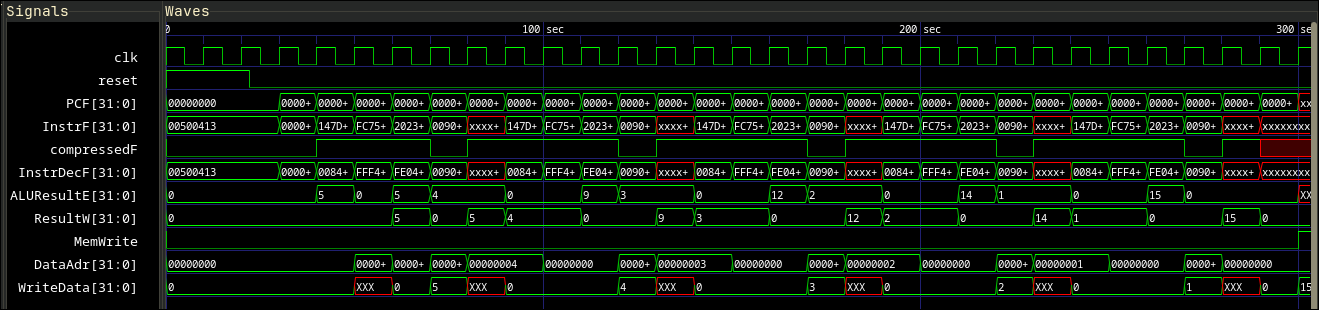
\includegraphics[width=\linewidth]{sumloop_waveform.png}
  \caption{Ejecucion del algoritmo \texttt{sumloop} ($5+4+3+2+1$). El
  \texttt{PCF} itera sobre el cuerpo del bucle
  (\texttt{0x8}$\to$\texttt{0xA}$\to$\texttt{0xC}$\to$\texttt{0x8}),
  \texttt{compressedF} se activa en las tres comprimidas, y \texttt{ALUResultE}
  acumula \texttt{5, 9, 12, 14, 15}.}
  \label{fig:sumloopwave}
\end{figure}

En la captura se observa:
\begin{itemize}[leftmargin=1.6em]
  \item \textbf{El bucle.} \texttt{PCF} vuelve a \texttt{0x8} tras cada
        \texttt{c.bnez} tomado, mientras el contador (en \texttt{ALUResultE},
        via \texttt{c.addi}) baja \texttt{5,4,3,2,1}.
  \item \textbf{Descompresion.} \texttt{InstrF} muestra la comprimida cruda
        (p.ej. \texttt{0x94A2} para \texttt{c.add}) e \texttt{InstrDecF} su
        expansion RV32I; la \texttt{c.bnez} \texttt{0xFC75} se expande al
        \texttt{bne} correspondiente.
  \item \textbf{La acumulacion.} \texttt{ResultW} muestra la suma parcial
        \texttt{5, 9, 12, 14, 15} conforme se ejecuta \texttt{c.add}.
  \item \textbf{Resultado final.} Al terminar el bucle, \texttt{MemWrite=1},
        \texttt{DataAdr=0} y \texttt{WriteData=15}: \texttt{Mem[0] = 15}.
\end{itemize}

\subsection{Comparativa de tamano y \textit{performance}}

Se compilo el mismo algoritmo en dos versiones: una que aprovecha las
comprimidas (\texttt{-march=rv32ic}) y otra forzada a 32 bits
(\texttt{-march=rv32i}, o \texttt{.option norvc}). Ambas producen exactamente
el mismo comportamiento, pero difieren en el tamano del codigo:

\begin{table}[H]
	\centering
	\small
	\begin{tabular}{@{}lccc@{}}
		\toprule
		\textbf{Version} & \textbf{Instrucciones} & \textbf{Bytes (\texttt{.text})} & \textbf{Reduccion} \\
		\midrule
		RV32I puro (32 bits)      & 6 $\times$ 4 B          & 24 & --- \\
		Con RVC (3 comprimidas)   & 3$\times$4 B + 3$\times$2 B & 18 & \textbf{25\,\%} \\
		\bottomrule
	\end{tabular}
	\caption{Tamano del algoritmo \texttt{sumloop} con y sin compresion.}
	\label{cuadro:comparativa}
\end{table}

Sobre el \textbf{tamano}, las tres instrucciones del cuerpo del bucle
(\texttt{c.add}, \texttt{c.addi}, \texttt{c.bnez}) ahorran 2~bytes cada una: de
24 a 18~bytes, un \textbf{25\,\% menos}. En programas reales, donde predominan
las operaciones que tienen equivalente comprimido, el ahorro tipico de RVC ronda
el 25--30\,\%.

Sobre el \textbf{\textit{performance}}, el numero de instrucciones ejecutadas y
de ciclos es \textbf{identico} en ambas versiones: tras la descompresion en
Fetch, el pipeline ve exactamente las mismas instrucciones RV32I y las ejecuta
en los mismos ciclos. Ademas, la \textbf{ventana deslizante es puramente
combinacional}, por lo que no anade ni un ciclo de reloj. La ganancia de RVC,
por tanto, no es de velocidad de ejecucion sino de \textbf{densidad de codigo}:
un programa mas pequeno cabe mejor en memoria y en la cache de instrucciones,
lo que en un sistema con cache real reduce los fallos y mejora el rendimiento de
forma indirecta.

\subsection{Validacion automatizada}

Cada familia de instrucciones se valido con un testbench propio, integrado a la
regresion completa. Todos los casos pasan (23 de 23, incluidos los 12 de la Parte
1 del proyecto):

\begin{center}
\small
\begin{tabular}{@{}lll@{}}
\toprule
\textbf{Prueba} & \textbf{Instrucciones} & \textbf{Resultado} \\
\midrule
\texttt{caddi}   & \texttt{c.addi} & \texttt{Mem[0]=8} \\
\texttt{cir}     & \texttt{c.lui, c.slli, c.add} & \texttt{Mem[0]=17, Mem[4]=4096} \\
\texttt{ca}      & \texttt{c.sub, c.xor, c.or, c.and} & \texttt{Mem[0..12]=2,6,14,8} \\
\texttt{cb}      & \texttt{c.srli, c.srai, c.andi} & \texttt{Mem[0..8]=10,-4,4} \\
\texttt{mul10}   & \texttt{c.slli, c.add} (mixto) & \texttt{Mem[0]=60} \\
\texttt{clsw}    & \texttt{c.lw, c.sw} & \texttt{Mem[96]=77, Mem[100]=77} \\
\texttt{clspsp}  & \texttt{c.lwsp, c.swsp} & \texttt{Mem[116]=55, Mem[4]=55} \\
\texttt{cbz}     & \texttt{c.beqz, c.bnez} & \texttt{Mem[0]=7} \\
\texttt{cj}      & \texttt{c.j, c.jal} & \texttt{Mem[0]=5} \\
\texttt{cjr}     & \texttt{c.jr, c.jalr} & \texttt{Mem[0]=9} \\
\texttt{sumloop} & algoritmo (bucle 16/32) & \texttt{Mem[0]=15} \\
\bottomrule
\end{tabular}
\end{center}

Los programas combinan instrucciones de 16 y 32 bits, y cada resultado coincide
con el valor esperado, confirmando que las 21 instrucciones comprimidas funcionan
correctamente sobre el procesador segmentado.

\end{document}
